\documentclass{ntuthesis}
%套件安裝處
\usepackage{times}
\usepackage{verbatim}
\usepackage{color}
\usepackage{url}
\usepackage{graphicx}
\usepackage{array}
\usepackage{wallpaper} 
\usepackage{titlesec}
\usepackage{indentfirst}
\usepackage{titletoc}
\usepackage{enumerate}
\usepackage{tikz}
\usepackage{amsmath}
\usepackage{xeCJK}
\usepackage{CJKnumb}
\usepackage{hyperref}
\usepackage{apacite}
\usepackage{multirow}

\defaultCJKfontfeatures{AutoFakeBold=1}
\usetikzlibrary{shapes, arrows}
% Using the tex-text mapping for ligatures etc.
\defaultfontfeatures{Mapping=tex-text}
% Set the default fonts 
\setmainfont{Times New Roman}
\setCJKmainfont{BiauKai}
% Your information goes here
% 存取論文相關資訊
% Syntax: \var{English}{Chinese}
\university{National Taiwan University}{國立臺灣大學}
\college{College of Engineering}{工學院}
\institute{Institute of Industrial Engineering}{工業工程學研究所}
\title{The Research of Parameters Optimization In a Textile Dyeing Process
}{紡織染色製程最佳化問題之研究}
\author{Sheng-Chieh Chen}{陳聖捷}
\studentid{R04546020}
\advisor{I-Hsuan Hong, Ph.D.}{洪一薰 博士}
\defenseyear{2017}{106}
\defensemonth{July}{7}
\defenseday{21}

\begin{document}
\let\cleardoublepage\clearpage
%台大浮水印位置設定
\CenterWallPaper{0.174}{watermark.pdf}
  \setlength{\wpXoffset}{6.1725cm}
  \setlength{\wpYoffset}{10.5225cm}
%封面設定
\frontmatter
\makecover
\titleformat{\chapter}{\centering\Huge\bfseries}{第\,\CJKnumber{\thechapter}\,章}{1em}{}
\titlecontents{chapter}[0em]
{}{\makebox[4.1em][l]
{第\CJKnumber{\thecontentslabel}章}}{}
{\titlerule*[0.7pc]{.}\contentspage}
% \makecertification
% acknowledgements為致謝
%\begin{acknowledgementszh}
感謝\ldots
\end{acknowledgementszh}


%!TEX root = ../thesis.tex
\begin{abstractzh}
本研究的主要目的為,
在已知染色製程參數以及染色表現因子的關聯下,
建構機能布染色製程參數優化模型,
並考量生產成本以及品質成本,
以達到有效降低成本以及提高品質的穩定程度。
本研究主要分成二個部分,
一部分探討染整製程參數優化技術,
由表現因子關聯分析所估計的製程參數,
建構成本相關的染整製程總成本模型、品質相關的染整製程穩定度模型,
以及與品質標準有直接關係的染整製程對色差異度模型。
另一個部分基於前面部分所建構的模型,
本研究以非線性規劃的Sequential Quadratic Programming (SQP)方法,
分別對三個非凸規劃問題的模型,求解非線性規劃問題,
藉由搜尋方法找出製程運作成本最低、品質穩定度最高
以及對色差異度最小的表現因子組合。
\\ \\關鍵字:非凸集合、非線性規劃、序列二次規劃、穩定度
\end{abstractzh}

\begin{abstracten}
This research is to develop the dyeing parameter optimization model for functional textiles based on the analysis of relationship between the manufacturing parameters in the dyeing process and the dyeing performance. The aim of this research is to minimize the total dyeing cost including the production and energy quality costs with the consideration of robustness measure and dyeing performance.
Based on the relationship the estimated process parameters, the first task is discussion of the dyeing parameter optimization for dyeing process total costs model, dyeing process robustness model with consideration of the quality and the quality model about the chromatic aberration. 
According to the models, we use Sequential Quadratic Programming (SQP) method to solve the non-convex programming problems and search the combination of the maximum robustness of quality and the minimum of process cost and chromatic aberration. 
\\ \\Keywords: non-convex, nonlinear, SQP, robust
\end{abstracten}
\renewcommand\contentsname{目錄}
\tableofcontents
\addcontentsline{toc}{chapter}{\contentsname}

\renewcommand{\figurename}{圖}
\renewcommand\listfigurename{圖目錄}
\newcommand{\loflabel}{圖}
\renewcommand{\numberline}[1]{\loflabel~#1\hspace*{1em}}
\listoffigures
\addcontentsline{toc}{chapter}{\listfigurename}

\renewcommand{\tablename}{表}
\renewcommand\listtablename{表目錄}
\newcommand{\lotlabel}{表}
\renewcommand{\numberline}[1]{\lotlabel~#1\hspace*{1em}}
\listoftables
\addcontentsline{toc}{chapter}{\listtablename}
\mainmatter
\setlength{\parindent}{2em}
% 主要文章位置
% Chapter 1
%!TEX root = ../thesis.tex
\chapter{介紹(主章結標題)}
\label{c:intro} %交互參照
近年來新興國家低成本紡織品紛紛興起\dots

為了達到在不影響品質下,有效降低染整過中不必要的浪費,並能選擇適合的製程參數因子,因此本研究的目的如下:(列舉)模式
\begin{enumerate}[(1)]
	\item 建立一個適合紡織業者經常使用的染整製程的最佳化模型框架。
	\item 為了建構模型框架,考量多種環境因子對於本研究的目標特性,找出提供效益最大的模型因子。
	\item 由最佳化求解方法求解環境因子建構的模型,得到高品質以及低成本的組合。
\end{enumerate}



% Chapter 2
%!TEX root = ../thesis.tex
\chapter{文獻探討}
\label{c:literat}
布料的染整加工程序被認定為一個高耗能型產業,由於從布料製作到染布進入裁切的過程當中會運用到大量的化學藥劑、水、升溫燃料及運作所需的電能,故在本研究當中,我們會藉由調整製程參數來降低能源及資源的使用量,進而減少在染布製成當中的總消耗成本。另外,我們也藉由調整製程參數來提高布料品質,而在品質與降低成本當中取得一個適當的平衡點為本研究的主要目的。本研究計畫的文獻回顧分為「染色製程參數與對色關聯性」及「染色製程參數優化技術」兩個部分,探討目前業界目前常用的參數組合以及,染色製成優化技術的趨勢。
%!TEX root = ../thesis.tex
\section{次章節標題}
\label{c:ch2.1}
染整製程的環境下,對於染布的均勻度及製程所造成的成本都會和許多的參數息息相關。但在建置成研究模型時,如果使用大量的參數可以找出較貼近於實際的模型,而且可以藉由此模型找出最好的解。
並且在染整過程中,有許多染色條件會影響到紡織物染後結果,譬如染料的組成、配方組合及染程的參數設計等。其中染料的組成會影響染料的上色速度,配方組合會影響助劑的用量等。而對於染色製程參數對染色結果的影響,染場技術人員仍停留於先前經驗法則所制定出的製程參數水平值,然後再以誤差法通過多次試打樣去嘗試找出符合品質製程之最佳值,不僅浪費太多的時間和成本在經驗學習上,這樣的製程參數穩健性也不高,很容易受現場製程變異的影響。
目前相關文獻,大多只探討顏色染料的組成對染色失敗率或成本的影響,以及配方的改變對紡織布料染色後的品質影響,反而對製程參數的最佳化研究卻鮮有著墨。例如\cite{Harada.etc}發現染浴pH值可以用來設定不同種類的反應染料之吸盡率與固著率。\cite{Guo.etc}在通過對棉紗染色的研究,發現透過助劑的前處理過程可增加其著色力度。\cite{Chen}探討了三種不同類型的常壓可燃型聚酯織維物,在三種不同的分散性染料之染色結果。\cite{Huang.etc}發現當使用不同比例的單體混合接枝成棉織物,施染後棉織物具有不同的色力度值。\shortcite{Jasper.etc}利用類神經網路從染料的光譜吸光度來預測染料的濃度。可以看出上述文獻所探討的幾乎都是染料的組成和配方組合對染色結果之影響。

在過去文獻提到以實驗設計選擇染整製程參數,當中大部分是以紡織廠的過去經驗或是其他文獻做為依據,利用某些製程參數以原先的模型參數為基準,再進行微調的方式來做改善。像是\cite{Harada.etc}表示酸鹼值及溫度等面向,對於吸收率及固色率具有一定程度上的影響。\cite{jy2007dyeing}表示在尼龍布料的染整製程中,藉由微調酸鹼值、升溫溫度的模式及機台噴嘴內的壓力到某特定的參數值,就可以降低染布出現染整顏色不均勻的發生情況。然而\cite{Etemadifar.etc}述說以前的文獻及工廠所做的實驗方法,基本上都是依照其他研究所提出的參數,藉由固定特定參數下更改想要測量的參數加以變動,藉此了解此特定參數是否有對製程有所一定程度的影響,
\cite{Wang.etc}提出供技術人員參考和控制的關鍵因子以達到染色的均勻性,包含pH值、浴比及溫度等因子。藉由這些因子,探究製程參數對染色品質的影響,以期提出關鍵因子,得到穩健性更高的製程參數設置,並預估相關製程參數和染色品質的關係曲面。至於細節,由於第一章範圍與限制當中說明,本研究著重於模型架構,以及其相對應之最佳化模型求解,實驗設計的細節就不再贅述。
%!TEX root = ../thesis.tex
\section{染色製程參數優化技術}
\label{c:ch2.2}

% Chapter 3
%!TEX root = ../thesis.tex
\chapter{紡織染色製程現況}
\label{c:description}
一般而言染色製程總成本分為生產成本及品質成本。生產成本包括染整過程中之水、電成本及實驗室先期的實驗成本,染整過程中,若想要提高良率,通常現場所需要的生產成本也隨之提高。另一項成本為品質成本,當良率下降時導致色差、顏色不均、波紋及固色率不到標準,未達對色率標準時,不良品需再經過漂洗、補色等流程或直接報廢,這些過程產生的成本稱為品質成本。當良率愈低也就是重複染整的次數相對變多,對此造成資源上及時間的浪費,因此品質成本大幅增加。但是相對的,如果良率提升,會使得品質成本下降,但卻會造成生產成本大幅增加。生產成本與品質成本可能的相對應關係如圖~\ref{fig:graph1}所示,但如果能夠找出能夠品質與成本兼具的染整製成組合,如圖~\ref{fig:graph1}中的最佳製程總成本的位置,則必須要跳脫過去常用的製程參數,才有可能達到,但在求得製程參數組合的過程中,只依靠回饋去搜尋,則需要大量的實驗成本才有可能達到。
\begin{figure} 
\centering  
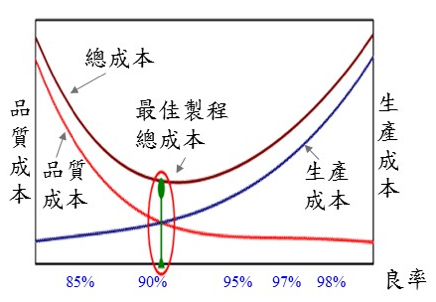
\includegraphics[width=8cm,height=6cm]{Graph/graph1.png}
\caption{染整製程品質成本及生產成本之關係曲線現況描述}
\label{fig:graph1}
\end{figure}
%!TEX root = ../thesis.tex
\section{染色製程描述}
\label{c:ch3.1}

%!TEX root = ../thesis.tex
\section{現況問題描述}
\label{c:ch3.2}

% Chapter 4
%!TEX root = ../thesis.tex
\chapter{染整製程模型建立}
\label{c:model}
前面章節敘述了介紹了文獻探討以及染整產業的現況,目前業者對於染整製程優化的部分以直觀的方法比較,學術上則是以啟發式演算法進行求解,如基因演算法\cite{Wu.etc},目前較少以非線性規劃的方法求解,故本章節主要詳細介紹如何建構染整製程最佳化模型。
%!TEX root = ../thesis.tex
\section{製程參數因子描述}
\label{c:ch4.1}
在染色製程中許多的因子會影響染後之染色表現因子,如染劑濃度、助劑濃度、初始pH值、浴比值、主泵浦速率、帶布輪速率、升溫速率、持溫溫度、水洗時間、皂洗升溫速率、皂洗持溫溫度、皂洗時間等。本研究計畫先聚焦於實驗室所能控制之製程參數:浴比值、升溫速率、持溫溫度、水洗時間、皂洗升溫速率、皂洗持溫溫度、皂洗時間等。染色製程參數與染色表現因子關聯分析,首先以統計實驗設計方法釐清關鍵之製程因子,並分析染色製程參數與染色表現因子關聯。但由於要得到各染色表現因子間的關係性必須透過實驗的方式,且也需考量實驗的成本,所以本研究由染整工廠建議及文獻當中,先針對特定幾項製程參數進行實驗。
\begin{figure} 
\centering  
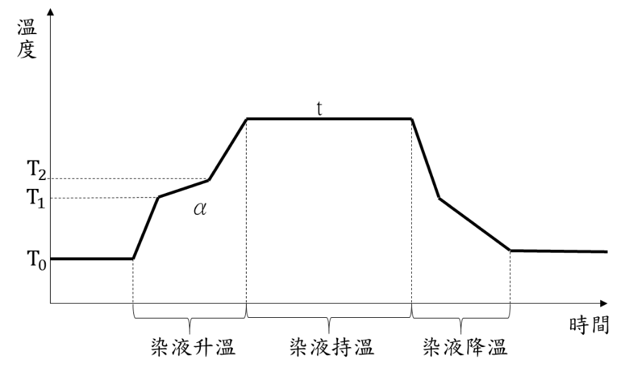
\includegraphics[width=12cm,height=8cm]{Graph/graph3.png}
\caption{聚酯纖維布料在染整階段時間與溫度關係}
\label{fig:graph3}
\end{figure}
圖\ref{fig:graph3}為第一階段染色製程,可以知道染色在升溫時,當溫度從常溫$T_0$到達$T_1$後就必須讓升溫速率降低,持續到升溫為$T_2$時在提升升溫速率。由於布料的性質,如果在染液升溫區間升溫太快,容易造成布料吸收不均的情況發生,因此在紡織業界也稱此區間為”危險區間“,經過此區間後。布料材質為聚酯纖維下必須要分三個階段來進行升溫,在圖\ref{fig:graph3}中為常溫,因為不同磅數的匹布在最高溫的設定會對染布吸收顏色能力上有一定的影響,所以及為我們設定的溫度參數。至於$\alpha$則為第二階段升溫時的升溫速率,由於$\alpha$的設定也會影響其他的製程參數,所以$\alpha$也納入我們設定的參數。而t為染布浸泡在染液中的持溫時間,時間越長吸收越好越穩定,但同時也會占用機台的產能,造成成本上升,故持溫時間也需列入考慮。最後由於升溫的速率及持溫的時間長短都會受到浴比值的影響,當浴比值越大則所需消耗的燃料成本就會相對較多,因此我們根據上列五個主要影響成本的因子做實驗設計,藉此來描繪各因子間與染色表現間的反應關係。

我們藉由分析以及與業者討論後,找出各因子間與染色表現因子或是成本間的反應關係。但由於在實驗室中,我們只能藉由檢測儀器檢測相關的染色表現因子,如色差值($\Delta E$)或固色力($K/S$),本研究計畫擬推估每次實驗所設定之製程參數,其相對應的染整過程所需耗用能源及水的總成本,如圖3.2
\begin{figure} 
\centering  
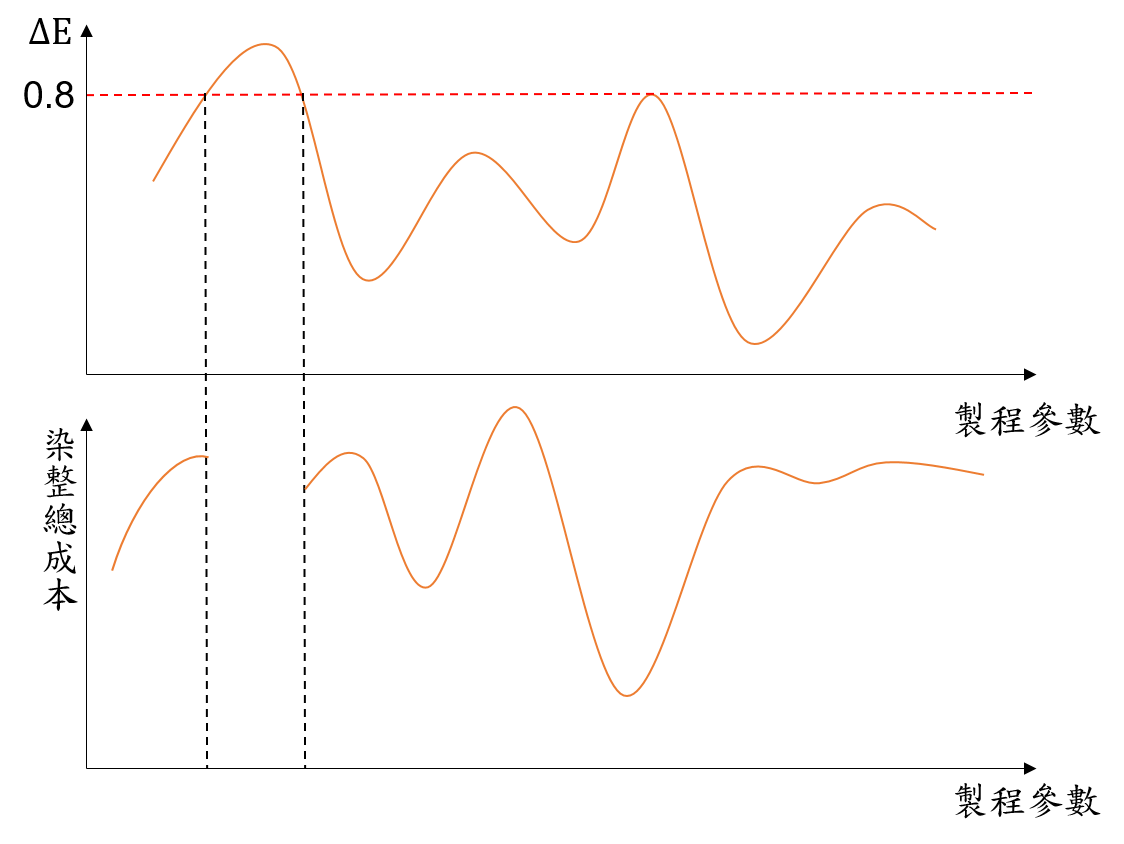
\includegraphics[width=12cm,height=10cm]{Graph/graph4.png}
\caption{聚染整總成本與色差值間的關係}
\label{fig:graph4}
\end{figure}

圖~\ref{fig:graph4}為成本與色差值間的關係示意圖,在圖~\ref{fig:graph4}的上半部為在固定染色配方下,描述各製程參數與色差值間的關係,從對應的製程參數設定,可推估染整廠實際所需花費的操作成本。而圖~\ref{fig:graph4}下半部則為染整製程總成本與製程參數間的關係。由圖~\ref{fig:graph4}可知下半部總成本有部分的區塊被截掉,原因是該製程參數所對應的色差值已經超出所規定的色差,故該區塊的製程總成本不列入成本的模型內。在本研究中由染色製程參數與染色表現因子關聯分析,能夠先分析出製程參數及色差值間的反應曲面,而在對應模型中,製程參數及總成本間的模型能夠互相對應,便能成功從色差值轉換為成本模型。

染色製程參數優化技術,以染色製程參數與染色表現因子關聯分析為輸入資訊,建構染色製程參數優化模型,描述上述製程因子對生產成本及品質成本之影響,搜尋製程總成本最低的製程參數組合。但由於「染色製程參數與染色表現因子關聯分析」需要分析各因子間的組合,就必須針對實際情況得到相對應的實驗數據,在實際染整工廠內進行實驗,對染整工廠來說成本是相當高,所以在「染色製程參數與染色表現因子關聯分析」中,只能從實驗室以5公克的布料來實驗。但從實驗結果得知相對的反應曲面,無法實際描繪出染整現場可能面對的製程參數變異,而造成品質成本的增加。再者,由於實驗室所做的實驗只能以5公克的布料來實驗,布的單次使用量非常的少,因此當製程參數在實驗室找出最佳製程參數結果,轉移到現場工廠內大量的布及大量的染料使用時,便可能會出現與實驗不同的結果。

在生產過程中除了考慮減少生產成本外,我們還需要考慮生產變異所造成的品質成本。在本研究中我們為了總成本最低的情況下符合品質外,我們還分別對品質成本搜尋最佳化結果,作為使用者調整生產以及品質間的平衡的依據,因此本研究將主要分成三個模型來表示第一個模型為生產成本模型(運作成本模型),第二個模型為品質穩健度模型,最後一個模型為品質模型($\Delta E$模型)。

%!TEX root = ../thesis.tex
\section{模型假設與符號表示}
\label{c:ch4.2}
根據上一小節所敘述的問題,本小節主要介紹染整製程參數優化模型當中,所需要的假設以及所需要使用的參數及變數符號。
\begin{enumerate}[(1)]
	\item 研究假設:
	\begin{enumerate}[i. ]
		\item 成本模型中,估計電的成本係數以及水的成本係數為定值,不依時間季節而變動。
		\item 由於實驗用的染缸材質,以至於熱散失所消耗的成本過低,所以熱散失成本並不列入考慮。
		\item 假設人為操作上並無差異。
		\item 由於本研究主要著重於影響較大的製程參數因子,故其他的環境參數因子假設為定值。
	\end{enumerate}
	\item 符號定義:
	\begin{enumerate}[]
		\item $EC$:電銷號總成本
		\item $WC$:水消耗總成本
		\item $TC$:機器佔用總時間成本
		\item $C_1$:每消耗一焦耳的電所換算的電消耗成本(台幣)
		\item $C_2$:每消耗一公斤的水所換算的水消耗成本(台幣)
		\item $C_3$:每佔用一分鐘的機台所換算的機器佔用成本(台幣)
		\item $E_i$:為主染程中第$i$段所需消耗的熱能(焦耳),$i=1\ldots3$
		\item $v$:從室溫到第一個目標溫度以及第一個目標溫度到第三個目標溫度的升溫速率($^\circ C/min$)
		\item $S$:為染液的熱容量
		\item $M$:為布的重量(公斤)
		\item $T_L$:室內溫度($^\circ C$)
		\item $T_H$:主染程中最高溫度($^\circ C$)
		\item $t_i$:為主染程中第$i$段機器所需使用的時間(分鐘),$i=1\ldots3$
		\item $c$:處理每公斤的廢水所需要的成本(台幣)
		\item $K$:染色過程所需要的換水次數
		\item $x_A$:在主染程中,從室溫開始升溫需要到達的第一個目標溫度($^\circ C$)
		\item $x_B$:在主染程中,第一個目標溫度以及第二個目標溫度之間的升溫速率($^\circ C/min$)
		\item $x_C$:在主染程中,從第一個目標溫度升溫需要到達的第二個目標溫度($^\circ C$)
		\item $x_D$:在主染程中,當溫度達到最高時,布料浸泡在染液中的時間(分鐘)
		\item $x_E$:在主染程中,每一公斤的布料所需要多少水量調和的浴比值
	\end{enumerate}
\end{enumerate}

%!TEX root = ../thesis.tex
\section{模型建立}
\label{c:ch4.3}
本研究中我們主要以三個模型進行介紹,分別為,成本模型、穩健度模型以及品質模型($\Delta E$模型),而這三個模型的主要差異在於其目標函式的設立,因此在本小節中我們將分別以這三個部分進行數學模式的建立。
\\ \textbf{運作成本模型}

成本目標函式主要分成電耗成本、水耗成本及機台占用時間成本,在此小節我們將根據此三個部分進行討論。
在電耗成本當中,我們以主染程在染布浸泡染液中,為了讓染布能有效吸收染液的顏色,故需要藉由提高溫度讓布料有效吸收顏料,因此在電耗成本的估算上,我們以染液加溫及持溫所需要消耗的熱能來估算機台所需提供的電耗,進而估算電耗成本,可得 \ref{eq:EC} 式:
\begin{equation}
	EC=C_1 \cdot \sum_i E_i, i=1 \dots 3
\label{eq:EC}
\end{equation}
其中為每焦耳所需要耗費的成本,為主染程前三段中第$i$段所需消耗的熱能,我們又可再將各階段的耗能依據主染程分成如 \ref{eq:EC_1} 式:
\begin{equation}
	\begin{array}{c}
	E_1=S \cdot M \cdot (x_A-T_L) \cdot x_E,\\
	E_2=S \cdot M \cdot (x_C-x_A) \cdot x_E,\\
	E_3=S \cdot M \cdot (T_H-x_C) \cdot x_E
	\end{array}
\label{eq:EC_1}
\end{equation}
由 \ref{eq:EC_1} 式子中可以知道第一段的熱能主要為升溫所需的熱能,第二段及第三段除了升溫的熱能。

水耗成本在染程中,水所消耗的部分除了染液所需要的耗水外,由於過程中需要多次的換水洗淨,故使用後的廢水也需要考量在內,而可得 \ref{eq:WC} 式:
\begin{equation}
	WC=(C_2+c) \cdot M \cdot K \cdot x_E
\label{eq:WC}
\end{equation}
其中為公斤的耗水量所需要的耗費成本,而$c$為每公斤的廢水所需要的處理成本,$K$為換水次數。由於除了主染程內的水需要更換外,還包含其他製程也需要換水,在耗水方面其他染程也會有所影響,故現階段這裡的水消耗成本利用總染程的水消耗成本來估算。

機台占用時間成本,每次在染色期間,由於布料需要時間吸收染料,機台就必須等待布料吸收完整後才能進入下一個階段,而機台在染程的階段,卻占用了機台可使用在別地方的時間成本及人力成本,所以我們根據機台在主染程估算的時間做為機台所被占用的時間,並乘上單位時間所需的成本做為我們的機台占用成本,並可得到 \ref{eq:TC} 式:
\begin{equation}
	TC=C_3 \cdot (\sum_i t_i + x_D), i=1\dots 3
\label{eq:TC}
\end{equation}
其中$C_3$為機台占用每分鐘所需的成本,而則為主染程第$i$階段的時間。
\\ \textbf{穩健度模型}

由前面章節提到,
,我們藉由前面實驗設計所得到$\Delta E$的函式,將函式根據各個因子做偏微分,並且平方後加總,值越大則代表該組合所在的位置並不穩定,反之則較為穩定,故我們將搜尋其最小化作為我們建構模型之一。製程參數因子關聯分析中,預估$\Delta E$迴歸式$f_{\Delta E}(x_A,x_B,x_C,x_D,x_E)$,為了找出其穩定的程度,我們藉由對此函式先分別進行對各因子的偏微分
\begin{equation*}
	\bigtriangledown f_{\Delta E}(x_A,x_B,x_C,x_D,x_E) = {
		\left[
			\begin{array}{c}
			\partial f_{\Delta E}(x_A,x_B,x_C,x_D,x_E)/\partial x_A\\
			\vdots\\
			\partial f_{\Delta E}(x_A,x_B,x_C,x_D,x_E)/\partial x_E\\
			\end{array}
		\right]
	}
\end{equation*}
,由此得到一組向量解,在這裡我們以$\bigtriangledown f_{\Delta E}$表示,其表示的意義為搜尋時,最佳化最快的方向,也可以由$\bigtriangledown f_{\Delta E}$觀察出此組解各自在該函式穩定的程度,為了將這些值統合起來以一個質的方式表示,找出對所有組合中找出最為穩定的解,故我們將取$(\bigtriangledown f_{\Delta E})^T \cdot (\bigtriangledown f_{\Delta E} )$,在此我們定義為$\bigtriangledown f_{\Delta E}$ norm的平方,作為我們簡化的依據,為了讓結果不會過於敏感故我們最後將$\bigtriangledown f_{\Delta E}$ norm的平方開根號,作為本研究中穩健度的指標。

根據上敘述整理後,我們將此目標函式的數學模式設立為 \ref{eq:robust} 式:
\begin{equation}
	f_{robust}(x_A,x_B,x_C,x_D,x_E) = \left[
			\sum_{i=A\dots E}\partial f_{\Delta E}(x_A,x_B,x_C,x_D,x_E)/\partial x_i)^2
		\right]^{1/2}
\label{eq:robust}
\end{equation}
\textbf{品質模型($\Delta E$模型)}

由前面介紹過$\Delta E$愈小則表示,與目標顏色的差距越低,所以當越小則代表我們的品質越高
,因此我們由染整製程參數因子關聯分析中得到$\Delta E$迴歸式$f_{\Delta E}(x_A,x_B,x_C,x_D,x_E)$,為了找出影響品質最大的參數因子組合,本研究根據紡織業者使用的Datacolor MATCH的數據,藉由關聯分析得到$\Delta E$迴歸式,由於$\Delta E$為主要的評判染色布料加工後是否為報廢品的依據,故我們以$\Delta E$的回歸模型為我們的品質模型。

由上面介紹了本研究根據染整製程參數所建構出的三個模型,我們將此三個目標函式整理為 \ref{eq:cost1} $
\sim$ \ref{eq:deltaE1} 式
\begin{equation}
	\begin{split}
	\min_{x_A,x_B,x_C,x_D,x_E} [C_1SM(T_H-T_L)+(C_2+c)MK]\cdot x_E+\\
	C_3 \cdot [(x_C-x_A)(v-x_B)/(v\cdot x_B) +(T_H-T_L)/v+x_D]
	\end{split}
\label{eq:cost1}
\end{equation}
\begin{equation}
	\min_{x_A,x_B,x_C,x_D,x_E} \left[
		\sum_{i=A\dots E}\partial f_{\Delta E}(x_A,x_B,x_C,x_D,x_E)/\partial x_i)^2
	\right]^{1/2}
\label{eq:robust1}
\end{equation}

\begin{equation}
	\min_{x_A,x_B,x_C,x_D,x_E} f_{\Delta E}(x_A,x_B,x_C,x_D,x_E)
\label{eq:deltaE1}
\end{equation}
而在限制式方面,基本上大同小異,以下為其三個目標函式所要配對的限制式,如 \ref{eq:constraint} 式:
\begin{equation}
	\begin{array}{c}
	A_{lower} \leq x_A \leq A_{upper},\\
	B_{lower} \leq x_B \leq B_{upper},\\
	C_{lower} \leq x_C \leq C_{upper},\\
	D_{lower} \leq x_D \leq D_{upper},\\
	E_{lower} \leq x_E \leq E_{upper},\\
	\Delta E_{lower} \leq f_{\Delta E} \leq \Delta E_{upper},\\
	K/S_{lower} \leq f_{K/S} \leq K/S_{upper}
	\end{array}
\label{eq:constraint}
\end{equation}
由式 \ref{eq:constraint} 中,$A_{lower}$為染整參數因子$x_A$的下屆值,而$A_{upper}$則為其上屆值,依此類推$\dots$,由前面三個目標函式 \ref{eq:cost1} $
\sim$ \ref{eq:deltaE1} 式分別與以上七個限制式,分別組合為前面所提到本研究所要探討的模型,架構以上模型後,可以發現本研究的目標函式以及限制式都為非線性的模式,在下面的章節當中,我們會介紹如何以非線性規劃求解的方法,去尋找這三個染整製程最佳化模型。
% Chapter 5
%!TEX root = ../thesis.tex
\chapter{染整製程參數優化方法}
\label{c:opt_method}
根據前面 \ref{c:ch3.1} 節,我們介紹了染整製程參數優化模型的建立,分別為運作成本模型、穩健度模型以及品質模型($\Delta E$模型),在 \ref{c:ch3.2} 我們會根據這三個模型分別進行最佳化求解。在本節當中我們分為三個部分討論,首先會先對模型環境進行描述,再針對此非線性模型提出符合條件的最佳化方法,最後介紹三個優化模型進行求解。
%!TEX root = ../thesis.tex
\section{模型描述}
\label{c:ch5.1}
接下來在本小節當中,我們分別對此三個模型進行轉換,以及模型環境上的描述。但在模型轉換前,我們先列出從Datacolor MATCH提供的資訊而預估的兩個品質控管模型的細節;由於我們從染整參數關聯分析當中,得到已知的$\Delta E$以及$K/S$的估計式,基本上兩者都為二次的函式,由於不同的環境會有不同的係數組合,故在本節當中,我們已通用式表示,如 \ref{eq:deltaEf} 式以及 \ref{eq:KSf} 式:
\begin{equation}
	\begin{array}{c}
	f_{\Delta E}(x_A,x_B,x_C,x_D,x_E)=\sum_i C_i\cdot x_i + \sum_i C_{ii}\cdot x_i^2+\sum_i\sum_j C_{ij}\cdot x_{i}\cdot x_{j},\\i=A,B\dots E,j=A,B\dots E , i\neq j
	\end{array}
\label{eq:deltaEf}
\end{equation}
\begin{equation}
	\begin{array}{c}
	f_{K/S}(x_A,x_B,x_C,x_D,x_E)=\sum_i C_i^{'}\cdot x_i+ \sum_i C_{ii}^{'}\cdot x_i^2+\sum_i\sum_j C_{ij}^{'}\cdot x_{i}\cdot x_{j},\\i=A,B\dots E,j=A,B\dots E,i\neq j
	\end{array}
\label{eq:KSf}
\end{equation}
\ref{eq:deltaEf}式以及 \ref{eq:KSf} 式,$C_{i}$以及$C_i^{'}$分別為$\Delta E$以及$K/S$一次因子的係數,而$C_{ii}$以及$C_{ii}^{'}$分別為$\Delta E$以及$K/S$二次因子的係數,$C_{ij}$以及$C_{ij}^{'}$分別為$\Delta E$以及$K/S$各因子交互作用係數。
\\ \textbf{運作成本最小化模型}

在 \ref{eq:cost1} 式中,我們可以知道此目標函式除了為非線性函式外,變數$x_B$在分母的位置,為了降低計算上的複雜度,我們以變數變換的方式將其轉換為,如下 \ref{eq:cost2} 式:
\begin{equation}
	\begin{split}
	\min_{x_A,x_B,t,x_D,x_E} [C_1SM(T_H-T_L)+(C_2+c)MK]\cdot x_E+\\
	C_3 \cdot [t\cdot (v-x_B)+(T_H-T_L)/v+x_D]
	\end{split}
\label{eq:cost2}
\end{equation}
由 \ref{eq:cost2} 式中,我們將設定一個新變數$t=(x_C-x_A)/x_B$其意義為,第一段升溫溫度到第二段升溫溫度所需花費的時間,由這樣的變數變換下,我們將\ref{eq:EC}式轉換為一個標準二次函式,如 \ref{eq:cost2} 式。

在變數變換時,為了將目標函數的複雜度將低,同時我們也會增加其變數以及限制式作為代價,因此在運作成本模型當中的目標函式,從原來的 \ref{eq:constraint} 式新增為,如 \ref{eq:constraint2} 式:
\begin{equation}
	\begin{array}{c}
	A_{lower} \leq x_A \leq A_{upper},\\
	B_{lower} \leq x_B \leq B_{upper},\\
	C_{lower} \leq x_C \leq C_{upper},\\
	D_{lower} \leq x_D \leq D_{upper},\\
	E_{lower} \leq x_E \leq E_{upper},\\
	(C_{lower}-A_{upper})/B_{upper} \leq t \leq (C_{upper}-A_{lower})/B_{lower},\\
	x_C-x_A-x_B\cdot t = 0,\\
	\Delta E_{lower} \leq f_{\Delta E} \leq \Delta E_{upper},\\
	K/S_{lower} \leq f_{K/S} \leq K/S_{upper}
	\end{array}
\label{eq:constraint2}
\end{equation}
由 \ref{eq:constraint2} 式中主要是多增加了兩個限制式,分別為$(C_{lower}-A_{upper})/B_{upper} \leq t \leq (C_{upper}-A{lower})/B_{lower}$以及$x_C-x_A-x_B\cdot t = 0$,前者為時間的範圍限制,後者則表示為與$x_A$以及$x_B$兩因子之間的關係,雖然額外增加了一個變數以及兩條限制,但 \ref{eq:constraint2} 中還是為二次不等式。
我們將轉型的目標函式以及不等式合併後,就成為了一個二次規劃中二次限制式的問題,也就是QCQP(Quadratic Constraints Quadratic Programming)問題。
\\\textbf{穩健度模型}

而在穩健度模型,同樣可以將模型轉化為二次函式,首先我們將 \ref{eq:deltaEf} 式帶入 \ref{eq:KSf} 式,再將目標函式取平方,如 \ref{eq:robust2} 式:
\begin{equation}
	\begin{array}{c}
	\min_{x_i} \sum_{i}[C_{i}+2C_{ii}\cdot x_i+\sum_j(C_{ij}+C_{ji})\cdot x_i]^{2},\\i=A,B\dots E,j=A,B\dots E , i\neq j
	\end{array}
\label{eq:robust2}
\end{equation}
而其限制函式一樣為 \ref{eq:constraint} 式,沒有額外的轉換,將 \ref{eq:robust2} 式與限制式 \ref{eq:constraint} 合併後,同樣為QCQP的問題。
\\\textbf{品質模型($\Delta E$模型)}

品質模型的目標函式以及限制式,不需要做任何轉換以及更改,合併後就是為QCQP問題。我們將 \ref{eq:deltaEf} 式帶入 \ref{eq:deltaE1} ,如 \ref{eq:deltaE2} 式:
\begin{equation}
	\begin{array}{c}
	\min_{x_i}\sum_i C_i\cdot x_i + \sum_i C_{ii}\cdot x_i^2+\sum_i\sum_j C_{ij}\cdot x_{i}\cdot x_{j},\\i=A,B\dots E,j=A,B\dots E , i\neq j
	\end{array}
\label{eq:deltaE2}
\end{equation}

%!TEX root = ../thesis.tex
\section{非線性最佳化方法}
\label{c:ch5.2}
從上一小節當中,我們介紹了染整製程參數優化模型三個主要,分別以運作成本最小化模型、穩定度模型以及品質模型($\Delta E$模型),並且轉化為QCQP問題的形式,接下來我們將導入序列二次規劃法(SQP,Sequential Quadratic Programming)方法並且介紹,搜尋最佳化問題的研究方法的理論原理,再針對本研究主要的以上三個模型進行求解介紹。
\\\textbf{序列二次規劃法介紹}

在\cite{Gill.etc}中表示,SQP方法在限制式以及目標函式為二次非線性的情況下被廣泛地使用,而且對於搜尋大範圍的非線性最佳化問題,是非常好用的方法,在本研究當中目標函式以及限制事皆為多維度非線性二次函式,所以以SQP方法將原問題重複簡化爲子問題,藉由搜尋子問題的最佳解作為下一參數組合的下一個移動的方向以及其距離,重複的迭代直到參數組合不再移動,就代表已經找到我們所需要的參數最佳解。

我們將原模型示意為,如 \ref{eq:exmodel} 式:
\begin{equation}
	\begin{array}{c}
	\min_{x} f(x) \\
	h(x)=0 \\
	g(x)\leq 0
	\end{array}
\label{eq:exmodel}
\end{equation}
目標函式以及限制式皆為非線性,我們可以將此非線性模型轉化為一子問題,在某一參數組合下以泰勒展開估計目標函式並將非線性的限制式線性化,如 \ref{eq:exmodel2} 式:
\begin{equation}
	\begin{array}{c}
	\min_{d} f(x^{k})+ \bigtriangledown f(x^{k})^{T}d+1/2\cdot d^{T}H(x^{k})d\\
	h(x^{k})+ \bigtriangledown h(x^{k})^{T}d=0\\
	g(x^{k})+ \bigtriangledown g(x^{k})^{T}d\leq 0
	\end{array}
\label{eq:exmodel2}
\end{equation}
由 \ref{eq:exmodel2} 式當中$x^{k}$為當前的參數組合,而$d$為一組向量,而下一代次的參數組合為$x^{k+1}=x^{k}+d$,當$x^{k+1}\approx x^{k}$時則找到最佳參數組合。
\\ \textbf{牛頓序列二次規劃法}

在 \cite{Gill.etc} 中有提到,SQP方法其中一個優勢是一個不太受限於可行區域的方法,儘管起始點不在可行區域,也同樣可以進行搜尋,但也有在模型的目標函式限性轉化時,可能會減弱其限制能力,因此我們會以Lagrange乘數法,將原限制式的資訊加入原目標函式內,再將其轉化為子問題求解,如 \ref{eq:exmodel3} 式:
\begin{equation}
	\begin{array}{c}
	\min_{d} \bigtriangledown L(x^{k},\lambda^{k},\mu^{k})^{T}d+1/2\cdot d^{T}\bigtriangledown^{2}L(x^{k},\lambda^{k},\mu^{k})d\\
	h(x^{k})+ \bigtriangledown h(x^{k})^{T}d=0\\
	g(x^{k})+ \bigtriangledown g(x^{k})^{T}d\leq 0
	\end{array}
\label{eq:exmodel3}
\end{equation}
因此在 \ref{eq:exmodel3} 我們做了些轉變,在目標函式中除了使用Lagrange乘數法,如 \ref{eq:exlagrange} 式:
\begin{equation}
L(x,\lambda,\mu)=f(x)-\lambda \cdot h(x)-\mu \cdot g(x)
\label{eq:exlagrange}
\end{equation}
還將常數的部分去掉,因為在子問題中的常數部分不會受到變數的影響,簡化了不必要的部份,在3.22式中$\lambda$以及$\mu$分別為等號限制以及不等號限制的Lagrange乘數,在 \ref{eq:exlagrange} 式的子問題我們可以從簡化後的QP問題做$d$的求解,接下來將介紹本研究中序列二次規劃法的演算。

在\cite{Nocedal.etc}一書,表示序列二次規劃法求取區域最佳解,在符合KKT條件下以牛頓法進行SQP求解,為了求得轉化後的子模型的變數向量$d$,首先在已知當前解$x^{k}$、$\lambda^k$以及$\mu^{k}$的目標函式,我們從Lagrange的條件下,假設\\
\begin{equation*}
	\Psi(x^{k},\lambda^{k})= \left[ 
	\begin{array}{c} 
		\bigtriangledown L(x^{k},\lambda^{k},\mu^{k}) \\
		h(x^{k}) \\
	\end{array}
	\right]=0
\end{equation*}
其中為了符合KKT條件,在非等號限制式的部分只能保留受約束的限制式(set of active),也就是當前解帶入非等號限制式時則等號會成立,為了達到同樣的效果,我們將原本的不等限制式的部分加上一個鬆弛變數(slack variable),讓限制式都以等式限制式的$h(x)$表示。接下來我們假設Jacobian為
\begin{equation*}
	J(x^{k},\lambda^{k})= \left[ 
	\begin{array}{cc} 
		\bigtriangledown^{2} L(x^{k},\lambda^{k}) & \bigtriangledown h(x^{k})\\
		\bigtriangledown h(x^{k})^{T} & 0 \\
	\end{array}
	\right]
\end{equation*}
為了得到下一代次的解$x^{k+1}$以及$\lambda^{k+1}$,其中
\begin{equation*}
	\begin{array}{c}
	x^{k+1}=x^{k}+d_x,\\
	\lambda^{k+1}=\lambda^{k}+d_{\lambda}
	\end{array}
\end{equation*}
最後我們從 \ref{eq:solequation} 式中得到子問題中的$d=(d_x,d_{\lambda})$
\begin{equation}
J(x^{k},\lambda^{k})\cdot d =\Psi(x^{k},\lambda^{k})
\label{eq:solequation}
\end{equation}
但在序列二次規劃法中以在符合Lagrange條件下的牛頓法計算最佳化問題時,必須符合以下幾個條件
\begin{enumerate}[(1)]
	\item 限制式的Jacobian必須是滿秩(full rank)
	\item $J(x^{k},\lambda^{k})$必須要保持正定,牛頓法才可使用
\end{enumerate}
由於以上兩個條件限制下,便會無法對原問題如果是非凸集合下的非線性二次規劃問題尋找最佳解,為了這個問題,在\cite{Nocedal.etc}一書說明,如遇到$J(x^{k},\lambda^{k})$無法維持正定時,則以擬牛頓法(quasi-newton method)則可以解決非凸集合下的非線性規劃問題。
\\ \textbf{擬牛頓法}

從原本的模型藉由SQP轉化爲QP的問題,如果當此子問題的Hessian矩陣為正定矩陣,則我們可以使用牛頓法,由於牛頓法搜尋最佳解的收斂速度很快,故可以作為求解的方法,但在實際上染整所估計得目標函式以及限制式,其Hessian矩陣不一定會是正定,有可能為半正定或者兩者都不是,當Hessian矩陣不是正定或是半正定時,則我們的問題就會是非凸規劃問題(Non-convex programming problems)
,則在這裡我們使用擬牛頓法(Quasi-newtons)和牛頓法比較下會比較適合。

在牛頓法當中,雖然收斂速度很快,但是卻存在了兩個問題,一個是在迭代過程中計算量過大問題以及Hessian矩陣必須保持正定,但如果問題為非凸規劃問題時,就無法使用牛頓法求解,擬牛頓法主要能夠在割線條件(Secant condition)下,找出逼近Hessian矩陣的估計矩陣,此估計矩陣為正定,故擬牛頓法可以解決牛頓法的問題,也就是除了解決計算量過大外,可以解抉非凸規劃問題。

在3.23式當中,$J(x^{k},\lambda^{k})$有可能無法維持正定,故我們以擬牛頓法來估計一個最接近$J(x^{k},\lambda^{k})$的矩陣$B_{k}$,在擬牛頓估計矩陣的方法有許多種,如:DFP (Davidon Fletcher Powell, DFP)方法、BFGS (Broyden Fletcher Goldfarb Shanno, BFGS)方法, Broyden等,而在\cite{Nocedal.etc}一書中說明了,目前使用擬牛頓法解決最佳化問題中,BFGS是效果較好且也較廣泛地使用的方法之一,故在本研究中也同樣以BFGS作為估計矩陣的方法,由於BFGS是使用迭代的方法,也就是$B_{k+1}=B_{k}+\Delta B_{k}$,由於起始的$B_{0}$通常為單位矩陣,故我們針對$\Delta B{k}$的部分進行說明,假設向量$y_k=\Psi(x^{k+1},\lambda^{k+1})-\Psi(x^{k},\lambda^{k})$而$s_{k}= - \alpha_{k} \cdot B_{k}^{-1} \cdot \Psi(x^{k},\lambda^{k})$其中$\alpha_{k}$為擬牛頓搜尋迭代過程中的步伐大小,通常我們以Line search的方法進行逼近,最後得到的步伐大小就為$\alpha_{k}$,而$x_{k+1}=x_{k}+s_{k}$,在符合割線條件下我們得到 \ref{eq:deltaB} 式
\begin{equation}
\Delta B_{k}=\frac{y_{k}y_{k}^{T}}{y_{k}^{T}s_{k}}+\frac{B_{k}s_{k}s_{k}^{T}B_{k}^{T}}{s_{k}^{T}B_{k}s_{k}}
\label{eq:deltaB}
\end{equation}
由 \ref{eq:deltaB} 式得到$B_{k+1}$後,進而計算下一個代次,直到$x_{k+1} \approx x_{k}$時則停止演算。

我們整理序列二次規劃法的演算流程,如圖 \ref{fig:flow3}
\begin{figure} 
\centering
%!TEX root = ../thesis.tex
\tikzstyle{endpoint} = [rectangle,draw,rounded corners, minimum width=7em, minimum height=2em,text centered, draw=black]

\tikzstyle{decision} = [diamond, draw, 
    text width=5em, text badly centered, node distance=3cm, inner sep=0pt]
\tikzstyle{block} = [rectangle, draw, 
    text width=7em, text centered, minimum height=2em]
\tikzstyle{line} = [draw, -latex']
    
\begin{tikzpicture}[node distance = 1.5cm, auto]
    % Place nodes
    \node [endpoint] (init) {給定初值};
    \node [block, below of=init] (identify) {確立搜尋方向};
    \node [block, below of=identify] (step) {計算步伐};
    \node [block, below of=step] (cal) {計算搜尋結果};
    \node [decision, below of=cal] (decide) {是否最佳};
    \node [endpoint, below of=decide,node distance=3cm] (con) {停止搜尋};
    \node [block, right of=cal,node distance=4cm] (update) {迭代資訊更新};
    % Draw edges
    \path [line] (init) -- (identify);
    \path [line] (identify) -- (step);
    \path [line] (step) -- (cal);
    \path [line] (cal) -- (decide);
    \path [line] (decide) -- node {Yes}(con);
    \path [line] (decide) -| node {No}(update);
    \path [line] (update) |- (identify);
\end{tikzpicture}
\caption{序列二次規劃演算流程圖}
\label{fig:flow3}
\end{figure}
在圖 \ref{fig:flow3} 首先我們會先給定起始值$x_{0}$、$\lambda_{0}$以及停止條件$\epsilon$,再來確立搜尋的方向$d_{k}=-B_{k}^{-1}\Psi_{k}$,確認方向後將給定值帶入後,以Line search方法計算$\alpha_{k}$,就會得到$s_{k}=\alpha_{k}d_{k}$以及$x^{k+1}=x^{k}+s_{k}$,最後判斷$s_{k}$是否小於$\epsilon$,如果是,則停止搜尋,反之則繼續將$y_{k}$以及$B_{k+1}$求出後,再回到確立搜尋方向繼續迭代。
%!TEX root = ../thesis.tex
\section{染整製程模型求解}
\label{c:ch5.3}
在上一小節當中,我們介紹了本研究的求解方法,而在本小節當中我們會序列二次規劃法套用到本研究主要三個模型當中,並根據圖3.3的序列二次規劃演算流程,搜尋此三個模型的最佳染整參數組合。
\\\textbf{運作成本最小化模型}

在進行演算流程前,我們先將模型進行轉化以及整理,由3.16式當中,首先我們藉由增加鬆弛變數(slack variable) $w_{ij}$將不等式型態轉為等式的型態$h_{i}(x)$,在第一行到第五行不等式中,將其轉換為
\begin{equation}
	\begin{array}{c}
	x_{i}-i_{upper}-w_{i0}=0,\\
	i_{lower}-x{i}-w_{i1}=0,\\
	i\in \{A,B,C,D,E\}
	\end{array}
\label{eq:hx1}
\end{equation}
由 \ref{eq:hx1} 式中我們從 \ref{eq:constraint2} 式中的前五行不等式的轉換下,我們得到$h_{1}(x) \sim h_{10}(x)$,在 \ref{eq:constraint2} 式的第六行不等式,我們將其轉換為 \ref{eq:hxt} 式而得到$h_{11}(x) \sim h_{12}(x)$
\begin{equation}
	\begin{array}{c}
	t-(C_{upper}-A_{lower})/B_{lower}-w_{t0}=0,\\
	(C_{lower}-A_{upper})/B_{upper}-t-w_{t1}=0
	\end{array}
\label{eq:hxt}
\end{equation}
而第七行則為$h_{13}(x)=x_C-x_A-x_B\cdot t$,最後把 \ref{eq:deltaEf} 及 \ref{eq:KSf}式帶入 \ref{eq:constraint2} 式中轉換,並得到$h_{14}(x) \sim h_{17}(x)$,如 \ref{eq:hx2} 式
\begin{equation}
	\begin{array}{c}
	\sum_i C_i\cdot x_i + \sum_i C_{ii}\cdot x_i^2+\sum_i\sum_j C_{ij}\cdot x_{i}\cdot x_{j}-\Delta E_{upper}-w_{\Delta E0}=0,\\
	\Delta E_{lower}-\sum_i C_i\cdot x_i + \sum_i C_{ii}\cdot x_i^2+\sum_i\sum_j C_{ij}\cdot x_{i}\cdot x_{j}-w_{\Delta E1}=0,\\
	\sum_i C_i^{'}\cdot x_i+ \sum_i C_{ii}^{'}\cdot x_i^2+\sum_i\sum_j C_{ij}^{'}\cdot x_{i}\cdot x_{j}-K/S_{upper}-w_{K/S0}=0,\\
	K/S_{lower}-\sum_i C_i^{'}\cdot x_i+ \sum_i C_{ii}^{'}\cdot x_i^2+\sum_i\sum_j C_{ij}^{'}\cdot x_{i}\cdot x_{j}-w_{K/S1}=0,\\
	i,j\in \{A,B,C,D,E\} , i\neq j
	\end{array}
\label{eq:hx2}
\end{equation}
因此我們可以從 \ref{eq:cost2} 式與上面轉換後的限制式合併後,得到 \ref{eq:cost3} 式
\begin{equation}
	\begin{split}
	L(x,t,\lambda)=[C_1SM(T_H-T_L)+(C_2+c)MK]\cdot x_E+\\
	C_3 \cdot [t\cdot (v-x_B) +(T_H-T_L)/v+x_D]-\sum_{i=1}^{17} \lambda_{i}\cdot h_{i}(x)
	\end{split}
\label{eq:cost3}
\end{equation}
並從 \ref{eq:cost3} 式推得$\bigtriangledown L(x,t,\lambda)$,如 \ref{eq:costg}式
\begin{equation}
\bigtriangledown L(x,\lambda)=\left[ 
	\begin{array}{c}
	\lambda_{2}-\lambda_{1}-(\lambda_{14}-\lambda_{15}) \frac{\partial f_{\Delta E}}{\partial x_{A}}-(\lambda_{16}-\lambda_{17}) \frac{\partial f_{K/S}}{\partial x_{A}} \\

	\lambda_{4}-\lambda_{3}-(\lambda_{14}-\lambda_{15}) \frac{\partial f_{\Delta E}}{\partial x_{B}}-(\lambda_{16}-\lambda_{17}) \frac{\partial f_{K/S}}{\partial x_{B}}+C_{3} \Delta T t/v \\

	\lambda_{6}-\lambda_{5}-(\lambda_{14}-\lambda_{15}) \frac{\partial f_{\Delta E}}{\partial x_{C}}-(\lambda_{16}-\lambda_{17}) \frac{\partial f_{K/S}}{\partial x_{C}} \\

	C_{3}+\lambda_{8}-\lambda_{7}-(\lambda_{14}-\lambda_{15}) \frac{\partial f_{\Delta E}}{\partial x_{D}}-(\lambda_{16}-\lambda_{17}) \frac{\partial f_{K/S}}{\partial x_{D}} \\

	Const+\lambda_{10}-\lambda_{9}-(\lambda_{14}-\lambda_{15}) \frac{\partial f_{\Delta E}}{\partial x_{E}}-(\lambda_{16}-\lambda_{17}) \frac{\partial f_{K/S}}{\partial x_{E}} \\

	\end{array}
	\right]
\label{eq:costg}
\end{equation}
其中$Const=[C_1SM(T_H-T_L)+(C_2+c)MK]$以及$\Delta T=(T_{H}-T_{L})$,而$\Delta E$和$K/S$估計式的偏微分分別為\\
\begin{equation*}
	\begin{array}{c}
		\frac{\partial f_{\Delta E}}{\partial x_{i}}=C_{i}+2C_{ii}x_{i}+(\sum_{i} C_{iA} x_{i}+\sum_{j} c_{Aj} x_{j}) \\
		\frac{\partial f_{K/S}}{\partial x_{i}}=C_{i}^{'}+2C_{ii}^{'}x_{i}+(\sum_{i} C_{iA}^{'} x_{i}+\sum_{j} c_{Aj}^{'} x_{j})\\
		i,j\in {A,B,C,D,E}
	\end{array}
\end{equation*}
再將$\bigtriangledown L(x,\lambda)$以及$h_{1}(x)\sim h_{17}(x)$得到$\Psi(x,\lambda)$以及$J(x,\lambda)$。
\\\textbf{穩健度模型}

在穩健度模型中,我們同樣先將模型進行轉化以及整理,由 \ref{eq:constraint} 式當中,首先我們藉由增加鬆弛變數$w_{ij}$將不等式型態轉為等式的型態$h_{i}(x)$,在第一行到第五行不等式中,與 \ref{eq:hx1} 式相同,便可得到$h_{1}(x) \sim h_{10}(x)$,最後把 \ref{eq:deltaEf} 及 \ref{eq:KSf} 帶入 \ref{eq:constraint} 式中轉換,並得到$h_{11}(x) \sim h_{14}(x)$,與 \ref{eq:hx2} 式相同,因此我們可以從 \ref{eq:robust2} 式與上面轉換後的限制式合併後,得到 \ref{eq:robust3} 式
\begin{equation}
	\begin{split}
	L(x,\lambda)=\sum_{i}[C_{i}+2C_{ii}\cdot x_i+\sum_j(C_{ij}+C_{ji})\cdot x_i]^{2}-\sum_{i=1}^{14} \lambda_{i}\cdot h_{i}(x)
	\end{split}
\label{eq:robust3}
\end{equation}
並從 \ref{eq:robust3} 式推得$\bigtriangledown L(x,t,\lambda)$,如 \ref{eq:robustg} 式 \newpage
\begin{equation}
\bigtriangledown L(x,\lambda)=\left[ 
	\begin{array}{c}
	\lambda_{2}-\lambda_{1}-(\lambda_{14}-\lambda_{15}+Const_{A}) \frac{\partial f_{\Delta E}}{\partial x_{A}}-(\lambda_{16}-\lambda_{17}) \frac{\partial f_{K/S}}{\partial x_{A}} \\

	\lambda_{4}-\lambda_{3}-(\lambda_{14}-\lambda_{15}+Const_{B}) \frac{\partial f_{\Delta E}}{\partial x_{B}}-(\lambda_{16}-\lambda_{17}) \frac{\partial f_{K/S}}{\partial x_{B}} \\

	\lambda_{6}-\lambda_{5}-(\lambda_{14}-\lambda_{15}+Const_{C}) \frac{\partial f_{\Delta E}}{\partial x_{C}}-(\lambda_{16}-\lambda_{17}) \frac{\partial f_{K/S}}{\partial x_{C}} \\

	\lambda_{8}-\lambda_{7}-(\lambda_{14}-\lambda_{15}+Const_{D}) \frac{\partial f_{\Delta E}}{\partial x_{D}}-(\lambda_{16}-\lambda_{17}) \frac{\partial f_{K/S}}{\partial x_{D}} \\

	\lambda_{10}-\lambda_{9}-(\lambda_{14}-\lambda_{15}+Const_{E}) \frac{\partial f_{\Delta E}}{\partial x_{E}}-(\lambda_{16}-\lambda_{17}) \frac{\partial f_{K/S}}{\partial x_{E}} 
	\end{array}
	\right]
\label{eq:robustg}
\end{equation}
其中$Const_{i}=4C_{ii}$而$i\in \{A,B,C,D,E\}$,再將$\bigtriangledown L(x,\lambda)$以及$h_{1}(x)\sim h_{14}(x)$得到$\Psi(x,\lambda)$以及$J(x,\lambda)$。
\\\textbf{品質模型($\Delta E$模型)}

品質模型($\Delta E$模型)中,我們同樣先將模型進行轉化以及整理,由 \ref{eq:constraint} 式當中,首先我們藉由增加鬆弛變數$w_{ij}$將不等式型態轉為等式的型態$h_{i}(x)$,在第一行到第五行不等式中,與 \ref{eq:hx1} 式相同,便可得到$h_{1}(x) \sim h_{10}(x)$,最後把 \ref{eq:deltaEf} 及 \ref{eq:KSf} 帶入 \ref{eq:constraint} 式中轉換,並得到$h_{11}(x) \sim h_{14}(x)$,與 \ref{eq:hx2} 式相同,因此我們可以從 \ref{eq:deltaE2} 式與上面轉換後的限制式合併後,得到 \ref{eq:deltaE3} 式
\begin{equation}
	\begin{split}
	L(x,\lambda)=\sum_i C_i\cdot x_i + \sum_i C_{ii}\cdot x_i^2+\sum_i\sum_j C_{ij}\cdot x_{i}\cdot x_{j}-\sum_{i=1}^{14} \lambda_{i}\cdot h_{i}(x)
	\end{split}
\label{eq:deltaE3}
\end{equation}
並從 \ref{eq:deltaE3} 式推得$\bigtriangledown L(x,t,\lambda)$,如 \ref{eq:deltaEg} 式
\begin{equation}
\bigtriangledown L(x,\lambda)=\left[ 
	\begin{array}{c}
	\lambda_{2}-\lambda_{1}-(\lambda_{14}-\lambda_{15}+Const_{A}) \frac{\partial f_{\Delta E}}{\partial x_{A}}-(\lambda_{16}-\lambda_{17}) \frac{\partial f_{K/S}}{\partial x_{A}} \\

	\lambda_{4}-\lambda_{3}-(\lambda_{14}-\lambda_{15}+Const_{B}) \frac{\partial f_{\Delta E}}{\partial x_{B}}-(\lambda_{16}-\lambda_{17}) \frac{\partial f_{K/S}}{\partial x_{B}} \\

	\lambda_{6}-\lambda_{5}-(\lambda_{14}-\lambda_{15}+Const_{C}) \frac{\partial f_{\Delta E}}{\partial x_{C}}-(\lambda_{16}-\lambda_{17}) \frac{\partial f_{K/S}}{\partial x_{C}} \\

	\lambda_{8}-\lambda_{7}-(\lambda_{14}-\lambda_{15}+Const_{D}) \frac{\partial f_{\Delta E}}{\partial x_{D}}-(\lambda_{16}-\lambda_{17}) \frac{\partial f_{K/S}}{\partial x_{D}} \\

	\lambda_{10}-\lambda_{9}-(\lambda_{14}-\lambda_{15}+Const_{E}) \frac{\partial f_{\Delta E}}{\partial x_{E}}-(\lambda_{16}-\lambda_{17}) \frac{\partial f_{K/S}}{\partial x_{E}} 
	\end{array}
	\right]
\label{eq:deltaEg}
\end{equation}
其中$Const_{i}=C_{i}+2C_{ii}x_{i}+\sum_{j} (C_{ij}+C_{ji})x_{j}$而$i,j\in \{A,B,C,D,E\},i\neq j$,再將$\bigtriangledown L(x,\lambda)$以及$h_{1}(x)\sim h_{14}(x)$得到$\Psi(x,\lambda)$以及$J(x,\lambda)$。

我們從三個染整製程模型進行計算後,我們開始圖 \ref{fig:flow3} 的演算步驟搜尋運作成本模型的最佳解。在給定初始值的步驟當中,雖然序列二次規劃對於初始解的選擇可以不限於可行解當中,但在本研究會根據紡織廠所限定的可行解範圍內隨機挑選,\cite{Nocedal.etc}也表示,由於序列二次規劃法在估計原模型問題時好的起始解對於好的起始解對於結果來說,也會比較精確,故起始組合$x_{0}$從經驗上選取一組較為常用的解作為起始組合,而起始的Lagrange乘數$\lambda_{0}$我們則根據KKT條件下,我們以
\begin{equation*}
\lambda^{0}=-[\bigtriangledown h(x^{0})^{T}\bigtriangledown h(x^{0})]^{-1}\bigtriangledown h(x^{0})^{T}\bigtriangledown f(x^{0})
\end{equation*}
作為乘數的起始值,此外我們還需要設定迭代停止的依據,本研究以$x^{k+1}-x^{k}\leq \epsilon$作為演算終止的依據,而$\epsilon$在這裡我們設定在$10^{-5}$,而起始估計矩陣$B_{0}$通常則以單位矩陣作為起始的估計矩陣,確定各個起始值後,我們將起始值根據不同的模型分別帶入3.29、3.31及3.33式後,再與當前的$B_{k}$帶入$d_{k}=-B_{k}^{-1}\Psi_{k}$便能得到搜尋的方向,將搜尋方向乘以步伐後得到$x^{k+1}=x^{k}+\alpha_{k}d_{x}$以及$\lambda^{k+1}=\lambda^{k}+\alpha_{k}d_{\lambda}$。

將得到的$x^{k+1}$以及$\lambda^{k+1}$帶回$L(x,\lambda)$後以線搜索(line search)的方法求取$\alpha_{k}$便可得到$x^{k+1}$以及$\lambda^{k+1}$的值,最後判斷$x^{k+1}-x^{k}\leq \epsilon$如果符合條件,則停止演算,最佳解即為運做成本模型的最佳染整製程參數組合,反之則繼續將$y_{k}$以及$B_{k+1}$求出後,再回到確立搜尋方向繼續迭代。
% Chapter 6
%!TEX root = ../thesis.tex
\chapter{數值分析}
\label{c:numerical}
在前面章節我們介紹並且架構了本研究三個核心模型,並介紹我們如何以非線性規劃方法中的序列二次規劃法,求解這三個模型的最佳製程參數組合;在數值分析章節,我們主要分為五個小節,前面兩個小節,主要介紹數值化模型以及以序列二次規劃法搜尋最佳數值解,第三個小節我們以其他搜尋染整製程最佳化文獻的方法,比較業界常用組合以及本研究所使用的方法,第四小節則比較其他參數組合與搜尋後的最佳組合之間的差異,第五小節則藉由其他參數的變動,觀察結果間的差異。


%!TEX root = ../thesis.tex
\section{模型數值化}
\label{c:ch6.1}
在本研究三個主要模型數值化前,本小節將介紹染色過程中的基本參數,但由於品質模型以及穩定度模型參數,從關聯分析中便可得到估計回歸式,故我們主要針對運作成本模型的參數,詳細介紹各個估計參數的數值,如表\ref{tab:table1}所示
\begin{enumerate}[(1)]
	\item \textbf{熱容量及熱傳導係數:}\\由於染液的水占較大的比例,且熱容量會比水還高,估計染液的熱容量以水的熱容量做為下限估計係數,也就是每公斤的水升溫一度所需要4200焦耳的熱量做為估計數值。同時目前在熱散失估計上同樣以水的熱傳導係數做為估計係數,為每分鐘一公尺深的染液下降一度所散失33.6焦耳的熱能做為估計數值。
	\item \textbf{常溫及最高溫:}\\由紡織廠估計一般常溫以25度為準,而最高溫則分為淺色染程及深色染程所需要的溫度,淺色染程中以110度做為最高溫度,而深色染程中以130度做為最高溫度。
	\item \textbf{單位電價:}\\由於台電提供每度的電價會依照所消耗的電量而做不同的調整,但在這裡目前以平均每度3元做為係數下限值的估計,每度電為1000瓦而一焦耳為3600千瓦$\cdot$秒,所以可以得知每焦耳所花費的費用為1/12,000,000元。
	\item \textbf{單位水價及廢水處理單價:}\\在這裡目前以每度水10元的定值設為係數估計,而一度水為1000公斤,故也可以說每公斤的水約為0.01元。而紡織廠也提出每公斤單位水價基本上以每公斤0.011元計算,而廢水處理則以每公斤0.035元的方式計價。
	\item \textbf{第一段及第三段升溫速率:}\\由於限制式內第二階段升溫速率不超過每分鐘上升4.5度,而且在第一階段及第三階段升溫速率有不可過慢,所以目前以每分鐘上升3度為估計速率。
	\item \textbf{機台占用成本:}\\機台占用成本可能根據廠商對於此種儀器在這些時間當中能夠有多少產能,做為估算占用機台時間的成本。由紡織廠提供現場的單位時間占用機台成本,在這裡目前以每分鐘所占用機台時間成本以每分鐘29元做為估計值。
\end{enumerate}
\begin{table}[!htbp]
	\caption{模型參數估計值對照表}
	\center
	\begin{tabular}{ccc}
\hline	
	\textbf{估計項目} & \textbf{估計係數} & \textbf{單位} \\ \hline \hline
	熱容量($S$) & 4200 & $J/{kg\cdot T}$ \\
	常溫($T_L$) & 25 & $^\circ C$ \\
	最高溫度($T_H$) & 110 & $^\circ C$ \\
	第一段及第三段升溫速率($v$) & 3 & $^\circ C/min$ \\
	布重($M$) & 400 & $kg$ \\
	換水成本($K$) & 12 & $times$ \\
	單位電價($C_{1}$) & 1/12000000 & $NTD/J$ \\
	單位水價($C_{2}$) & 0.011 & $NTD/kg$ \\ 
	機台佔用成本($C_{3}$) & 29 & $NTD/min$ \\
	單位廢水成本($c$) & 0.035 & $NTD/kg$ \\
\hline
\end{tabular}
	\label{tab:table1}
\end{table}
\newpage
在表\ref{tab:table1}中的估計參數,與實際情況會根據不同的紡織廠的環境有所不同,再加上表中的參數我們假設電價以及水價不會隨著季節的變動而不同,也就是設定為平均定值,但經由與紡織產業討論後,並不會對模型造成影響;除了運作成本外,還有與紡織產業討論後得到每個參數因子的上下屆值,如表\ref{tab:table2}
\begin{table}
	\caption{染整參數因子上下界值表}
	\center
	\newcommand{\tabincell}[2]{\begin{tabular}{@{}#1@{}}#2\end{tabular}}  
\begin{tabular}{cccccc}
\hline	
	參數範圍 & \tabincell{c}{第一段目標\\溫度($^\circ C$)} & 
	\tabincell{c}{第二段升溫\\速率($^\circ C/min$)} & 
	\tabincell{c}{第三段目標\\溫度($^\circ C$)} & 
	\tabincell{c}{持溫時間\\($min$)} & 
	{浴比值} \\ 
	\hline \hline
	下界值 & 51 & 1.2 & 76 & 11 & 14\\
	上界值 & 61 & 1.8 & 86 & 19 & 26\\
\hline
\end{tabular}
	\label{tab:table2}
\end{table}
其中,分別為$x_A$、$x_B$、$x_C$、$x_D$以及$x_E$的上下界值。
\\ \textbf{運作成本數值最小化模型}\\
從理論上的模型架構以及方法套用,到本章節要討論,當實際的參數帶入理論模型中,是否可以得到比傳統經驗更優的結果,接下來我們會將理論模型數值化,再針對數值化過後的結果進行求解,以及與傳統比較各個模型中的優劣。
將表\ref{tab:table1}代入變數轉換後的運作成本模型,我們以\ref{model:cost}式表示
	\begin{equation}
	\begin{array}{c}
	\min_{x_A,x_B,x_C,x_D,x_E} \{ 820.7+19x_D+232.7x_E+29t+9.7x_Bt \} \\
	51 \leq x_A \leq 61,\\
	1.2 \leq x_B \leq 1.8,\\
	76 \leq x_C \leq 86,\\
	11 \leq x_D \leq 19,\\
	14 \leq x_E \leq 26,\\
	8.3 \leq t \leq 29.2,\\
	x_C-x_A-x_B\cdot t = 0,\\
	0 \leq f_{\Delta E}(x_A,x_B,x_C,x_D,x_E) \leq 0.8,\\
	95 \leq f_{K/S}(x_A,x_B,x_C,x_D,x_E) \leq 105
	\end{array}
	\label{model:cost}
\end{equation}
從上面式子中,可以觀察到運作成本模型的目標函式都為正數,參數因子愈小,則運作成本就愈小,但在限制式中有對品質進行限制,在求解中就不會那麼的直觀了。
\\ \textbf{穩定度數值模型}\\
從染整製程參數關聯性分析,以推估後的$(\Delta E's\ norm)^2$結果帶入回歸模型,我們以\ref{model:robust}式表示
\begin{equation}
	\begin{array}{c}
	\min_{x_A,x_B,x_C,x_D,x_E} \{ 
	(4.87-0.015z_A-0.17x_B-0.038x_C-0.029x_D)^2+\\
	(-0.015x_B+0.00014x_E)^2+(-0.038x_B+0.0027x_E)^2+\\
	(-0.029x_B-0.0011x_E)^2+(-0.45697+0.000148x_A+\\
	0.00271x_C-0.0011x_D+0.011x_E)^2 \} \\
	51 \leq x_A \leq 61,\\
	1.2 \leq x_B \leq 1.8,\\
	76 \leq x_C \leq 86,\\
	11 \leq x_D \leq 19,\\
	14 \leq x_E \leq 26,\\
	0 \leq f_{\Delta E}(x_A,x_B,x_C,x_D,x_E) \leq 0.8,\\
	95 \leq f_{K/S}(x_A,x_B,x_C,x_D,x_E) \leq 105
	\end{array}
	\label{model:robust}
	\hfill
\end{equation}
\textbf{品質數值模型}\\
從染整製程參數關聯性分析,以推估後的$\Delta E$結果帶入回歸模型,我們以\ref{model:deltaE}式表示
\begin{equation}
	\begin{array}{c}
	\min_{x_A,x_B,x_C,x_D,x_E} \{ 2.54 + 4.87x_B - 0.46x_E - 0.015x_Ax_B + \\ 
	0.00015x_Ax_E - 0.038x_Bx_C - 0.029x_Bx_D + 0.0027x_Cx_D - 0.0011x_Dx_E - \\
	0.086x_B^2 + 0.0056x_E^2 \} \\
	51 \leq x_A \leq 61,\\
	1.2 \leq x_B \leq 1.8,\\
	76 \leq x_C \leq 86,\\
	11 \leq x_D \leq 19,\\
	14 \leq x_E \leq 26,\\
	0 \leq f_{\Delta E}(x_A,x_B,x_C,x_D,x_E) \leq 0.8,\\
	95 \leq f_{K/S}(x_A,x_B,x_C,x_D,x_E) \leq 105
	\end{array}
	\label{model:deltaE}
	\hfill
\end{equation}
至於限制式中,兩個主要的品質指標,由估計後得到的$\Delta E$以及$K/S$數值函式分別為$f_{\Delta E}$估計函式
\begin{equation*}
	\begin{split}
	f_{\Delta E}(x_A,x_B,x_C,x_D,x_E)=2.54 + 4.87x_B - 0.46x_E - \\
	0.015x_Ax_B + 0.00015x_Ax_E - 0.038x_Bx_C - 0.029x_Bx_D + \\
	0.0027x_Cx_D - 0.0011x_Dx_E - 0.086x_B^2 + 0.0056x_E^2 
	\end{split}
\end{equation*}
以及$f_{K/S}$估計函式
\begin{equation*}
	\begin{array}{c}
	f_{K/S}(x_A,x_B,x_C,x_D,x_E)=-57.72+4.46x_A-36.52x_B+3.69x_D+3.51x_E+\\
	0.25x_Ax_B-0.042x_Ax_C-0.029x_Ax_D-0.019x_Ax_E+
	0.15x_Bx_C+0.36x_Bx_D+\\
	0.085x_Bx_E-0.022x_Cx_D-0.022x_Cx_E-0.0019x_Dx_E-0.0027x_A^2+\\
	0.82x_B^2+0.018x_C^2-0.026x_D^2-0.025x_E^2 
	\end{array}
\end{equation*}
得到數值化後的模型從\ref{model:cost}式$\sim$ \ref{model:deltaE}式後,在下一小節我們以序列二次規劃法對數值化的模型進行求解。
%!TEX root = ../thesis.tex
\section{染整製程數值求解}
\label{c:6.2}
在前面數值模型建立中,我們帶入了數值化參數後,得到 \ref{model:cost}式$\sim$ \ref{model:deltaE}式,再者我們經由序列二次規劃法求解,在本研究我們使用python套件中的pyOpt套件SLSQP方法,針對本研究三個主要的模型進行最佳化搜尋。

在\cite{Perez.etc}表示pyOpt是一個專門去解決有限制式的非線性規劃問題,而其中slsqp就是一個有效解決序列二次規劃方法的演算法之一,經過演算後,則表\ref{tab:table6}到表\ref{tab:table4}為經過序列二次規劃法的搜尋後,分別將運作成本模型、穩定度模型以及品質成本模型的搜尋結果分別列出

\begin{table}[!htbp]
	\caption{SQP方法搜尋運作成本模型最佳化結果表}
	\center
	%!TEX root = ../thesis.tex
%Cost
\begin{tabular}{ccccc}
\hline
\multicolumn{5}{c}{Objective function of operation cost: 5022.44(NTD)}\\
\multicolumn{5}{c}{Variables (c-continuous, i-integer, d-discrete):} \\
\hline
Name & Type & Value & Lower Bound & Upper Bound \\
\hline \hline
$x_A$ & c & 52.1 & 51 & 61 \\
$x_B$ & c & 1.20 & 1.2 & 1.8 \\
$x_C$ & c & 75.9 & 76 & 86 \\
$x_D$ & c & 15.4 & 11 & 19 \\
$x_E$ & c & 13.9 & 14 & 26 \\
\hline
\end{tabular}
	\label{tab:table6}
\end{table}

從表\ref{tab:table6}中,由於在實際紡織產業中溫度的調節、浴比值以及時間的調節,無法控制到整數以下的部分,而調節速率最多也只能調解至小數點下一位,因此我們從此組合當中調整為$[x_A,x_B,x_C,x_D,x_E]=[52,1.2,76,15,14]$而分別得到的結果為,運作成本為5044台幣、穩健度為0.558而$\Delta E$為0.775。

\begin{table}[!htbp]
	\caption{SQP方法搜尋穩健度模型最佳化結果表}
	\center
	%!TEX root = ../thesis.tex
%Robust
\begin{tabular}{ccccc}
\hline
\multicolumn{5}{c}{Objective function of robust: 0.0065}\\
\multicolumn{5}{c}{Variables (c-continuous, i-integer, d-discrete):} \\
\hline
Name & Type & Value & Lower Bound & Upper Bound \\
\hline \hline
$x_A$ & c & 59.9 & 51 & 61 \\
$x_B$ & c & 1.20 & 1.2 & 1.8 \\ 
$x_C$ & c & 85.2 & 76 & 86 \\
$x_D$ & c & 18.8 & 11 & 19 \\
$x_E$ & c & 20.5 & 14 & 26 \\
\hline
\end{tabular}
	\label{tab:table5}
\end{table}

從表\ref{tab:table5}中,同樣由於在實際紡織產業中溫度的調節、浴比值以及時間的調節,無法控制到整數以下的部分,而調節速率最多也只能調解至小數點下一位,因此我們從此組合當中調整為$[x_A,x_B,x_C,x_D,x_E]=[59,1.2,86,18,20]$而分別得到的結果為,運作成本為6561台幣、穩健度為0.061而$\Delta E$為0.225。

\begin{table}[!htbp]
	\caption{SQP方法搜尋品質模型最佳化結果表}
	\center
	%!TEX root = ../thesis.tex
%Delta E
\begin{tabular}{ccccc}
\hline
\multicolumn{5}{c}{Objective function of quality: 0.0401336}\\
\multicolumn{5}{c}{Variables (c-continuous, i-integer, d-discrete):} \\
\hline
Name & Type & Value & Lower Bound & Upper Bound \\
\hline \hline
$x_A$ & c & 61.0 & 51 & 61 \\
$x_B$ & c & 1.20 & 1.2 & 1.8 \\
$x_C$ & c & 78.4 & 76 & 86 \\
$x_D$ & c & 19.0 & 11 & 19 \\
$x_E$ & c & 24.5 & 14 & 26 \\
\hline
\end{tabular}
	\label{tab:table4}
\end{table}

從表\ref{tab:table4}中,同樣由於在實際紡織產業中溫度的調節、浴比值以及時間的調節,無法控制到整數以下的部分,而調節速率最多也只能調解至小數點下一位,因此我們從此組合當中調整為$[x_A,x_B,x_C,x_D,x_E]=[61,1.2,78,19,25]$而分別得到的結果為,運作成本為7545台幣、穩健度為0.255而$\Delta E$為0.042。

我們將以上的搜尋結果整理後如表\ref{tab:table3},將上述的最佳化模型參數組合表現相對應的結果,並從表中最佳化數值比較模型之間的最佳參數組合以及業界常用的染整製程參數組合的差異。
\begin{table}[!htbp]
	\caption{模型最佳化結果與業界常用製程參數對照表}
	\center
	%!TEX root = ../thesis.tex
\begin{tabular}{ccccccccc}
\hline
\multirow{2}{*}{Items} &
\multicolumn{5}{c}{Factors} &
\multicolumn{3}{c}{\multirow{1}{*}{Result}} \\
\cline{2-9}
  & $x_A$ & $x_B$ & $x_C$ & $x_D$ & $x_E$ & Cost & Robust & $\Delta E$ \\
\hline\hline
最小化成本 & 52 & 1.2 & 76 & 16 & 14 & 5044 & 0.558 & 0.775 \\ 
穩定度最佳化 & 59 & 1.2 & 86 & 18 & 20 & 6561 & 0.061 & 0.225 \\ 
品質最佳化 & 61 & 1.2 & 78 & 19 & 25 & 7545 & 0.255 & 0.042 \\ 
業界常用 & 56 & 1.5 & 81 & 15 & 20 & 6454 & 0.288 & 0.488 \\
\hline
\end{tabular}
	\label{tab:table3}
\end{table}
%!TEX root = ../thesis.tex
\section{方法比較}
\label{c:ch6.3}
在\cite{Wu.etc}表示,在紡織染色過程中所消耗的成本,其中主要包括原料、助劑以及廢水處理等,搜尋原料上的成本最佳化,在方法上使用基因演算法(GA, Genetic Algorithm),作為搜尋具限制式非線性規劃的主要搜尋方法,而在本研究當中,則是以序列二次規劃法分別搜尋成本以及品質的最佳解;在這個章節中,我們將使用基因演算法,分別搜尋本研究所建構的三個主要模型的最佳解,並且比較本研究所提的序列二次規劃法以及業界常用參數之間的差異。

%!TEX root = ../thesis.tex
\subsection{基因演算法概述}
\label{c:ch6.3.1}
基因演算法的核心理念主要可以回溯到1859年達爾文(Charles Darwin)提到「物競天擇,適者生存」的演化及淘汰概念,仿效自然界生物遺傳進化之天性,以適應該環境之生存型態,在1975年,此電腦模擬物種生存模式的演算法-基因演算法(GA, Genetic Algorithms),由\cite{holland1975adaptation}等人提出基因演算法概念。

在\shortcite{ritzel1994using}提到近幾年,基因演算法對於複雜的非線性規劃問題,具有良好的求解能力,\cite{goldberg1988genetic}表示基因演算法具有下列幾點優良的特性
\begin{enumerate}[(1)]
	\item 為了避免陷入區域最佳解,基因演算法會同時以多個點搜尋而不是單點做最佳化,因此可避免陷入區域的最佳解。
	\item 搜尋過程以機率的方式代替明確的規則,將問題引導至最佳解,故任何問題皆適用。
	\item 不需要繁瑣的數學計算,單純以適應函式作為優劣的評判。
\end{enumerate}

在本研究我們以\cite{Wu.etc}所使用的典型基因演算法中,介紹演算法的核心流程;基因演算是模擬自然界的演化程序,包括有複製(reproduction)、交配(crossover)與突變(mutation)等\dots,由於基因演算法是模擬基因的演化過程,其演化程序包括,複製、交配以及突變,從上一代到這一代的演化流程中染色體有可能會對自己進行「複製」以延續自己的序列組合,或者會與其他染色體進行「交配」,再下一代次中,有可能得到較好的配對結果成為下一代次,最後在交配以及複製期間有可能會產生「突變」的染色體,因此有可能產生比原本的基因更好的結果。

%!TEX root = ../thesis.tex
\subsection{基因演算法架構及求解}
\label{c:ch6.3.2}
從上一章節介紹了基因演算法的核心概念後,本章將介紹典型基因演算法的演算流程,如圖\ref{fig:flow4}所表示
\begin{figure}[!htb]
\center
%!TEX root = ../thesis.tex
\tikzstyle{endpoint} = [rectangle,draw,rounded corners, minimum width=7em, minimum height=2em,text centered, draw=black]
\tikzstyle{decision} = [diamond, draw, 
    text width=5em, text badly centered, node distance=3cm, inner sep=0pt]
\tikzstyle{block} = [rectangle, draw, 
    text width=7em, text centered, minimum height=2em]
\tikzstyle{line} = [draw, -latex']
    
\begin{tikzpicture}[node distance = 1.5cm, auto]
    % Place nodes
    \node [endpoint] (init) {隨機產生染色體};
    \node [block, below of=init] (fitness) {計算適應函數};
    \node [decision, below of=fitness] (decide) {是否滿足終止條件};
    \node [endpoint, below of=decide,node distance=3cm] (sol) {求得最佳解};
    \node [block, right of=decide,node distance=4cm] (reprod) {複製};
    \node [block, below of=reprod] (cross) {交配};
    \node [block, below of=cross] (mutate) {突變};
    % Draw edges
    \path [line] (init) -- (fitness);
    \path [line] (fitness) -- (decide);
    \path [line] (decide) -- node {Yes}(sol);
    \path [line] (decide) -- node {No}(reprod);
    \path [line] (reprod) -- (cross);
    \path [line] (cross) -- (mutate);
    \draw [line] (mutate) -- +(2,0) -- +(2,6) -- +(-2.4,6);
\end{tikzpicture}
\caption{基因演算法流程圖}
\label{fig:flow4}
\end{figure}
我們將從圖\ref{fig:flow4}逐步介紹基因演算流程圖
\begin{enumerate}[]
\item \textbf{隨機產生染色體:}\\
染色體(chromosome)代表一組可行解,在本研究當中為各個染整製程因子的組合,而在選定起始解當時通常我們會隨機的選定五個因子的值。
\item \textbf{產生適應函數:}\\
適應函數(fitness function)通常代表每一組染色體的優劣程度依據,在本研究當中目標函式就是每一組染整製程是否好壞的依據。
\item \textbf{滿足終止條件:}\\
終止條件通常會設定固定的遺傳代次(generation times),當到達迭代的次數則演算停止,以目前的結果作為最佳解,或者設定此次的最佳解與前一次的最佳解之間的誤差不超過某個微小值,為演算停止條件。
\item \textbf{複製:}\\
複製的過程當通常會選擇適應函數結果較好的染色體作為複製的對象,在本研究當中主要都以最小化作為搜尋的方向,故會挑選適應函數較小者為複製對象。
\item \textbf{交配:}\\
會從當代的染色體兩兩互相生成下一代的染色體稱為交配行為,而在交配過程當中會在當代的兩個染色體互相交換部份因子結果,例如在本研究當中會交換兩組參數因子中的前兩個因子,作為下一代次的染色體。
\item \textbf{突變:}\\
會在當代的染色體中機率性的選擇染色體內的某些組合因子,進行數值的變化,而在本研究當中為了不讓其搜尋過程容易掉入區域最佳解當中,會機率性的對五個因子做數值的變化,以增加搜索的可能性。
\end{enumerate}

在瞭解基因演算法基本架構後,我們將從\cite{Wu.etc}所使用的基因演算法,搜尋本研究所設置的三個主要的模型的最佳解,不過在求解之前由於前面章節提到,評判染色體的優劣主要依據適應函式的值,但在模型當中還需要考慮限制條件,而\cite{Wu.etc}使用Penalty方法,將限制式轉化為懲罰函式再將它併入目標函式,讓適應函式同時擁有目標函式以及限制的資訊,如\ref{eq:fitness}式,其中的Penalty函式$p(x)$在可行解時則懲罰值為0,反之則為懲罰函數值,$\Delta b(x)$為超出限制範圍的限制式,而$\Delta b^{nef}(x)$為接近可行解的閥值,如\ref{eq:penalty}式
\begin{equation}
F(x)=f(x)+p(x)
\label{eq:fitness}
\end{equation}
\begin{equation}
p(x)=
	\begin{cases}
	0,x\in feasible\ solution\\
	\sum_{i}^{m} \bigl(\frac{(\Delta b_{i}(x))}{\Delta b_{i}^{nef}(x)}\bigr)^{2}\\
	\end{cases}
\label{eq:penalty}
\end{equation}
在設定適應函式後,我們選擇\cite{rainville2012deap}中所提到的開放式資源,由於使用上較為穩定,且容易取得及使用,因此將套用python的Deap套件裡的基因演算方法求解,並根據\cite{Wu.etc}中的設定,將交配比率設為四分之一以及突變率設定為0.2,每一個代次染色體數設定為300個,並將迭代次數設定為500次,由演算過後如圖\ref{fig:GAopt}為三個主要模型各自的收斂狀況圖
\begin{figure}[!htb]
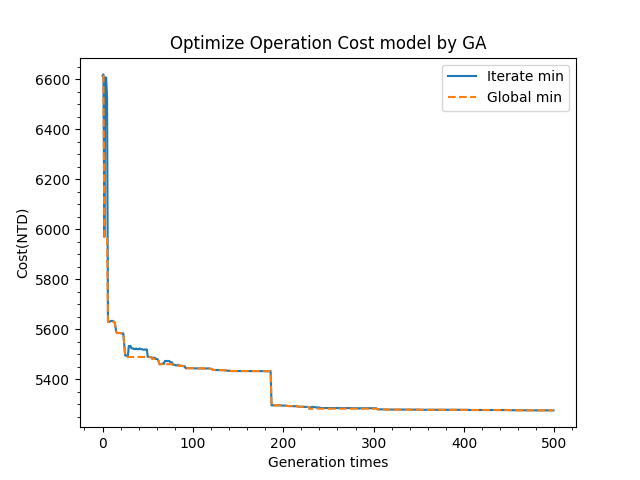
\includegraphics[width=8cm,height=6cm]{Graph/GAcost.png}
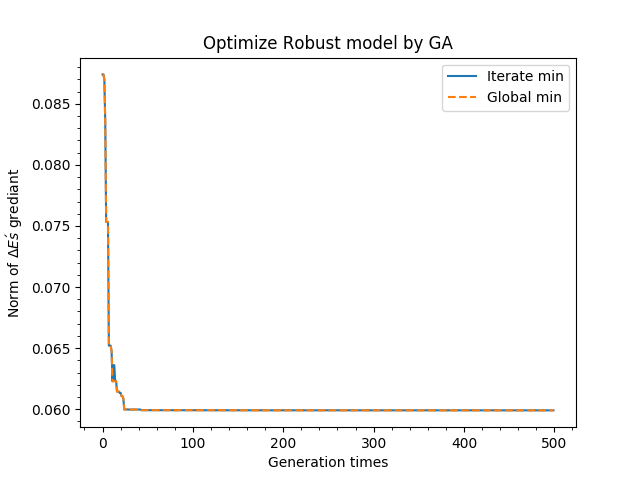
\includegraphics[width=8cm,height=6cm]{Graph/GARobust.png}
\center
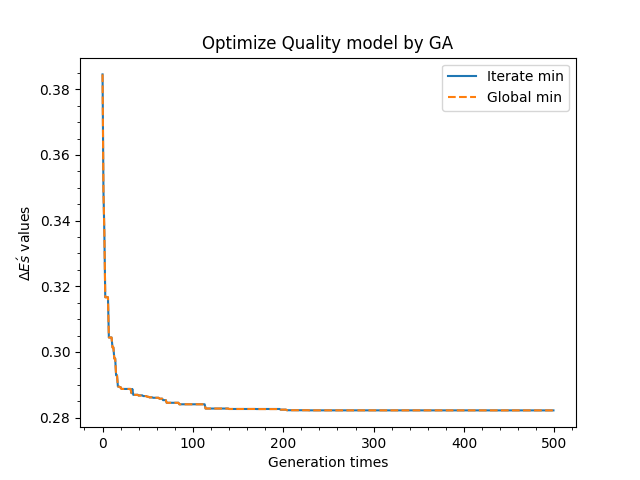
\includegraphics[width=8cm,height=6cm]{Graph/GADeltaE.png}
\caption{GA演算法搜尋各個模型最佳化收斂過程圖}
\label{fig:GAopt}
\end{figure}
\\由圖\ref{fig:GAopt}(左上)以GA演算法求解運作成本最小化模型,成本最佳解可以達到5275元,圖\ref{fig:GAopt}(右上)以GA演算法求解穩定度模型,其最佳解可達到約0.06,而圖\ref{fig:GAopt}(下)為品質成本的收斂過程圖,其$\Delta E$可達0.28,為了將得到的結果調整為符合實際紡織產業所能控制的範疇,如表\ref{tab:table7}將各個搜尋結果調整後分別套用至每個目標函數,便可比較製程參數組合間的差異。
\begin{table}[!htbp]
	\caption{基因演算法模型最佳化結果表}
	\center
	%!TEX root = ../thesis.tex
\begin{tabular}{ccccccccc}
\hline
\multirow{2}{*}{Items} &
\multicolumn{5}{c}{Factors} &
\multicolumn{3}{c}{\multirow{1}{*}{Result}} \\
\cline{2-9}
  & $x_A$ & $x_B$ & $x_C$ & $x_D$ & $x_E$ & Cost & Robust & $\Delta E$ \\
\hline\hline
最小化成本 & 51 & 1.3 & 76 & 18 & 15 & 5368 & 0.49 & 0.63 \\ 
穩定度最佳化 & 59 & 1.2 & 86 & 19 & 20 & 6590 & 0.065 & 0.168 \\ 
品質最佳化 & 61 & 1.2 & 82 & 19 & 23 & 7163 & 0.115 & 0.086 \\ 
\hline
\end{tabular}
	\label{tab:table7}
\end{table}





%!TEX root = ../thesis.tex
\section{最佳化參數組合與其他業界常用組合比較}
\label{c:ch6.4}
在這個小節當中,主要分別以本研究的最佳解方法以及可行範圍內隨機抽樣的樣本與業界常用的組合,相互比較並探討研究的方法在其他解中的優劣;在前面的小節,我們從模型數值化到序列二次規劃法以及基因演算法得到模型各自的最佳解與業界常用的組合,整理合併後得到表\ref{tab:table3}以及表\ref{tab:table7},但為了與其他可能會出現在業者所制定的染整製程參數組合比較,我們則從可行區域中提供幾組解作為比較的參數組合。
\begin{table}[!htbp]
	\caption{最佳化組合與其他業界常用組合比較表}
	\center
	%!TEX root = ../thesis.tex
\begin{tabular}{cccccccccc}
\hline
\multirow{2}{*}{Method} &
\multirow{2}{*}{Items} &
\multicolumn{5}{c}{Factors} &
\multicolumn{3}{c}{\multirow{1}{*}{Result}} \\
\cline{3-10}
  & &$x_A$ & $x_B$ & $x_C$ & $x_D$ & $x_E$ & Cost & Robust & $\Delta E$ \\
\hline\hline
GA演算法 & 最小化成本 & 51 & 1.3 & 76 & 18 & 15 & 5368 & 0.49 & 0.63 \\ 
& 穩定度最佳化 & 59 & 1.2 & 86 & 19 & 20 & 6590 & 0.065 & 0.168 \\ 
& 品質最佳化 & 61 & 1.2 & 82 & 19 & 23 & 7163 & 0.115 & 0.086 \\
\\
SQP方法 & 最小化成本 & 52 & 1.2 & 76 & 16 & 14 & 5044 & 0.558 & 0.775 \\ 
& 穩定度最佳化 & 59 & 1.2 & 86 & 18 & 20 & 6561 & 0.061 & 0.225 \\ 
& 品質最佳化 & 61 & 1.2 & 78 & 19 & 25 & 7545 & 0.255 & 0.042 \\ 
\\
隨機樣本 & 樣本一 & 54 & 1.4 & 79 & 14 & 22 & 6888 & 0.432 & 0.528 \\ 
& 樣本二 & 54 & 1.4 & 83 & 14 & 22 & 6975 & 0.285 & 0.557 \\ 
& 樣本三 & 54 & 1.4 & 83 & 16 & 22 & 7033 & 0.229 & 0.426 \\
& 樣本四 & 54 & 1.6 & 79 & 14 & 22 & 6888 & 0.399 & 0.611 \\ 
& 樣本五 & 54 & 1.6 & 79 & 16 & 22 & 6946 & 0.342 & 0.468 \\ 
& 樣本六 & 54 & 1.6 & 83 & 14 & 22 & 6975 & 0.254 & 0.609 \\ 
& 樣本七 & 54 & 1.6 & 83 & 16 & 22 & 7033 & 0.198 & 0.467 \\ 
\\
長期經驗 & 業界常用 & 56 & 1.5 & 81 & 15 & 20 & 6454 & 0.288 & 0.488 \\
\hline
\end{tabular}
	\label{tab:table8}
\end{table}

本研究以隨機抽樣的方式,搭配出不同的32種參數組合,但由於必須限制在$\Delta E$低於0.8以及$K/S$介於95到105之間,所以實際可行的隨機組合只有得到部分幾組,並將隨機的製程參數組合分別帶入各個目標函式後,如表\ref{tab:table8},將樣本的結果以及表\ref{tab:table3}和表\ref{tab:table7}合併後進行比較;從表\ref{tab:table8}可以觀察到,使用序列二次規劃法以及GA演算法搜尋的最佳解,在搜尋各自的項目上與其他的製程參數組合比較,是相對優秀的,說明此兩種方法在解決染整製程最佳化問題都能找到有效的區域最佳解;那麼在比較此兩種方法中,可以看出序列二次規劃法相對應的最佳化結果,都比基因演算法的結果再好一些,而且計算上更快速一些,故在表\ref{tab:table8}中,序列二次規劃法較基因演算法好一些,不過為了探討本研究提出的方法在整體上是否可以成功的替代業界常用的組合,我們必須從業界所提供的的其他資訊以及假設作為本研究整體評估的考量。

業界常用的製程參數組合,套用到實際的大染缸中,業者表示會有15\%的染布會與目標間存在差異,所以在$\Delta E$超過0.8時染布就需要重染或報廢,因此我們假設整體的報廢成本為失敗機率的等比級數總和乘以單次染布的運作成本,則我們假設評估整體的總成本為運作成本以及平均報廢成本的總和,而業界常用組合的平均總成本約為$6454\div (1-0.15)\simeq 7593$元。

業界常用參數是由長期的經驗法則所得來的結果,而且實際紡織業者提供一天所使用的染缸約160缸,故我們假設業界常用參數組合所呈現的$\Delta E$是符合平均數為0.488,及變異數未知的常態分配假設,雖然變異數未知,但我們從業者提供的資訊知道當超過$\Delta E$為0.8時,則失敗率為0.15中可推得其變異數為$[(0.8-0.488)/1.04]^2 = 0.09$;同樣的在這裡我們也假設其他的製程參數組合也符合平均數為各自的$\Delta E$,變異數為未知的常態分配,且通常越穩定的製程參數其$\Delta E$的變異會越小,故在這裡我們假設製程參數的變異數比與穩定度是成一般反比的關係,由以上這些假設條件下,我們便可以得到各組合的總成本,如表\ref{tab:table9}所示。
\newpage
\begin{table}
	\caption{最佳化組合與其他業界常用組合估計總成本比較表}
	\center
	%!TEX root = ../thesis.tex
\begin{tabular}{cccccc}
\hline
\multirow{2}{*}{Method}&
\multirow{2}{*}{Items} &
\multicolumn{4}{c}{Result} \\
\cline{3-6}
 & & Average & Variance & Failure rate & Total cost \\
\hline\hline
GA演算法 & 最小化成本 & 0.63 & 0.153 & 33.2\% & 8036 \\ 
& 穩定度最佳化 & 0.168 & 0.020 & 0.0005\% & 6590 \\ 
& 品質最佳化 & 0.086 & 0.036 & 0.0083\% & 7164 \\ 
\\
 SQP方法 & 最小化成本 & 0.775 & 0.174 & 48.0\% & 9700 \\ 
& 穩定度最佳化 & 0.225 & 0.019 & 0.0016\% & 6561 \\ 
& 品質最佳化 & 0.042 & 0.079 & 0.36\% & 7572 \\ 
\\
隨機樣本 & 樣本一 & 0.528 & 0.135 & 22.9\% & 8933\\ 
& 樣本二 & 0.557 & 0.089 & 20.7\% & 8795 \\ 
& 樣本三 & 0.426 & 0.072 & 8.1\% & 7652 \\
& 樣本四 & 0.611 & 0.125 & 29.6\% & 9784 \\ 
& 樣本五 & 0.468 & 0.107 & 15.5\% & 8220 \\ 
& 樣本六 & 0.609 & 0.079 & 24.9\% & 9287 \\ 
& 樣本七 & 0.467 & 0.062 & 9.0\% & 7728 \\ 
\\
長期經驗 & 業界常用 & 0.488 & 0.09 & 15\% & 7593 \\
\hline
\end{tabular}
	\label{tab:table9}
\end{table}

從表\ref{tab:table9}中,雖然隨機樣本的參數組合中的樣本三對業界常用組合較為穩定以及品質較高,但單次估計總成本卻比較高,可見業界常用組合是普遍在其他隨機樣本中確實是比較好的,而本研究的穩定度最佳化參數組合,以及使用基因演算法中的穩定度最佳化組合,則在估計總成本中比業界常用成本更低;雖然基因演算法穩定度結果與本研究方法差異不大,但是從綜合成本可量下,可看出本研究的方法還是稍微好一些,故在本研究的方法估計的綜合考量下,運作成本最佳組合以及品質最佳組合,雖然以該項目作為比較依據都比基因演算法好,但綜合評估下的成本卻比較高一些,故在選擇上業者需要自行評估哪一個模型比較符合當下需求,就本研究來說,建議使用SQP得到的穩定度模型最佳解是最好的選擇。

% \input{Chapter_6/section5}
% \input{Chapter_6/section6}
% Chapter 7
%!TEX root = ../thesis.tex
\chapter{結論}
\label{c:con}
本研究主要探討染色製程最佳化問題,從大略介紹機能布料對於現今世界的發展性,進而討論藉由降低紡織業在染色過程中的成本,提高紡織產業的利潤;為了有效降製程成本,我們數次拜訪業者,並由化驗室得來的實驗數據進行多項分析後,最後我們使用了五個對於染色過程中具有較大影響力的五個染整製程因子,作為本研究建置模型的決策變數,並根據這些製程參數的特性分別建置運作成本最小化模型、穩定度模型以及品質模型($\Delta E$模型),並藉由序列二次規劃法作為本研究的最佳化方法,分別對三個模型搜尋最佳解,因此分別得到模型的製程參數最佳組合;在數據分析中我們將其他文獻所使用的方法做為比較的對象,以基因演算法針對本研究的三個模型分別求解,得到的製程參數組合做為對照組合,另外我們還從可行區域內隨機抽取其他製程參數組合,最後將所有的製程參數組合與業界常用的組合互相比較。

在數據分析,在我們的假設下得知,序列二次規劃法中的穩定度最佳化模型所求得的製程參數組合,與其他的製程參數組合互相比較下,品質較好且較為穩定且所需要花費的運作成本差異不大,如果以每年250個工作天以及每天需要染整160缸染布下,約可以節省報廢或重染成本約每年三千多萬台幣,對於業者來說是相當可觀的成本花費。

本研究中主要只有探討五個具有顯著的影響成本、品質,以及業者有興趣的製程參數,並且根據運作成本以及品質進行求解以及數值分析,但實際的染整製成參數多達數十種,如在未來有機會能夠再與業者合作,可增加製程參數的種類以及增加實際現場的實驗數據,增加模型的可信度,並可以導入成本導向以及品質導向的目標合併,如多目標方法,在多製程參數下求取成本以及品質之間的最佳平衡點,除了為業者減少報廢成本外還能有效降低其他的成本。

\appendix
\backmatter
%參考文獻
\renewcommand\bibname{參考文獻}
%\addcontentsline{toc}{chapter}{\bibname}
% \bibliographystyle{abbrv}
\bibliographystyle{apacite}
\bibliography{thesis}
\end{document}
